\chapter{GPU内存超额配置的管理框架}
\label{chap:ETC}

本章针对内存超额配置导致的严重性能损失问题,介绍了一种内存超额配置管理框架。
\ref{sec:etcintroduction}节总体介绍了本章工作。
\ref{sec:etcrelated}节和\ref{background}节介绍了内存超额配置管理框架的相关工作及其研究背景。
\ref{sec:etcexplore}节介绍了一些设计探索及获得的经验。
\ref{sec:etcfeature}节研究了GPGPU应用程序的访存特性,为\ref{sec:etcdesign}节介绍的内存超额配置管理框架提供了设计依据。
\ref{sec:etcexperiment}节介绍了实验方法和实验结果,表明本章介绍的框架能够有效提升内存超额配置下应用程序的性能。
最后,\ref{sec:etcconclusion}节对全章进行了总结。


\section{引言}
\label{sec:etcintroduction}

随着面向高性能计算的应用程序对密集型计算的需求以及程序员对高可编程性需求的不断增加~\upcite{programmingguide,amd-hsa},如今图像处理器已经成为高性能计算领域首选的计算平台。
然而,想要使得应用程序发挥出最大的性能,依然要求程序员手动调整代码来适应GPU的系统硬件结构并满足内存容量的要求~\upcite{vijaykumar2016zorua}。
随着GPGPU应用程序的工作数据集不断增大~\upcite{kwon2018case,Rhu:2016:VVD:3195638.3195660,realizingIBM,meng2017training},有限地GPU内存容量已经成为影响硬件设计和程序性能的首要瓶颈~\upcite{rhu2018compressing,Rhu:2016:VVD:3195638.3195660,tianhao-hpca16}。

如今内存虚拟化技术不断演化进步,GPGPU程序可以通过虚拟化技术更加容易地扩展在线工作数据集(Working Set),使之可以在超出GPU内存物理容量的情况下工作~\upcite{abhishek-ispass16,spectlb,pichai-asplos14,tlb-consistency,amd-io-virt,intel-io-virt,ausavarungnirun2017mosaic,Ausavarungnirun:2018:MRG:3173162.3173169,powers-hpca14}。
现代GPU配备了\emph{统一内存空间}和\emph{实时按需取页}功能~\upcite{lindholm,pascal,volta},这些新的特性使得开发者不再需要手动地管理数据在CPU内存和GPU内存之间移动。
但是当一个GPU应用程序的工作数据集超出了内存的物理容量时(即内存超额配置时),旧数据必须被逐出,为能取新数据。
我们在一个真实GPU系统的测试显示,当内存超额配置时,GPGPU应用程序会遭受巨大的性能损失,有时甚至发生宕机。

通过程序员的软件优化,能够缓解一部分内存超额配置导致的性能损失~\upcite{sakharnykh2016beyond,unifiedmemorycuda6,maximizing,unifiedmemory2017,unifiedmemory2018}。
例如,程序员可以将只读数据从CPU内存复制到GPU内存而不是简单的迁移。
当应用程序需要更多空间存放新数据时,可以直接丢弃这些暂时不用的只读数据,而无需通过传统的数据页逐出方法,将数据写回到CPU的内存。
程序员可以将预取请求和逐出请求并行同步执行,新请求的数据无需等待内存逐出操作,有效地减少了延迟。
但是,采用软件优化方法来降低内存超额配置导致的性能损失有几个明显缺陷。
首先,软件方法要求程序员能够直接分清数据是否为只读数据;
其次,程序员必须理解并利用好成千上万条线程的局部性特征,手动地将不同地数据页映射到CPU或GPU的内存;
最后,程序员需要手动地在CPU和GPU内存之间迁移数据。
这些缺陷在云计算环境里会变得更加明显,因为共享一个GPU的虚拟机用户无法知道其他用户的应用程序的在线工作数据集大小,即无法预测超额配置的程度,难以对内存超额配置情况进行软件优化。
因此,设计一种对应用透明的机制来降低内存超额配置开销的需求非常迫切。

我们观察到利用当前GPGPU应用程序的两个关键特性可以更好地管理好超额配置的内存。
首先,内存超额配置带来的性能损失大小取决于不同应用程序的不同访存特性。
根据GPU内存的数据页访问是否具有可预测性,本章大致将应用程序分为\texttt{规则应用程序}和\texttt{非规则应用程序};
第二,内存超额配置开销的来源与程序类型相关。内存抖动(Thrashing),即持续地在CPU和GPU内存之间来回迁移数据页,是非规则程序的内存超额配置开销的最主要来源。
而较高的数据页逐出延迟则是规则程序在内存超额配置情况下的主要开销来源。
本章还发现同一个应用程序不同的GPU内核函数若存在数据共享,则会进一步降低GPU内存超额配置的性能。

基于这些特性,本章提出了一种叫ETC的内存超额配置管理框架。
该框架以一种对应用程序透明的方式来降低内存超额配置开销。
ETC第一步是高效自动地将应用程序划分为三类,包括数据不共享的规则应用程序、数据共享的规则应用程序以及非规则的应用程序。
之后ETC会基于应用程序的类型选择最有效的策略组合来缓解内存超额配置导致的性能损失。
ETC集成了多个模块,它们协同工作可以有效掩藏或减少内存超额配置带来的开销,主要包括:

(1)一个应用划分器,能够通过测量的访存合并系数来检测并判断应用程序的类型;

(2)一种策略引擎,能够基于应用程序类型选择并采用最合适的策略;

(3)一种主动数据页逐出技术,针对规则应用程序,提前主动逐出无用的数据页,为之后要请求的数据页腾出物理空间;

(4)一种内存感知的并行度控制策略,针对非规则应用程序,通过降低线程级并行来减少有效在线工作数据集;

(5)一种内存压缩引擎,能够为应用程序有效提高可用存储空间。



\section{相关工作}
\label{sec:etcrelated}
在我们知晓的范围内,本章的工作是第一个提出应用透明的软硬件结合解决方案,针对不同应用程序的类别采用最有效的技术组合来解决内存超额配置的问题。
本章调查了之前的工作,包括
(1)提供GPU上的统一虚拟内存支持相关工作;
(2)降低内存超额配置开销的相关工作;
(3)实现良好的线程级并行度的相关工作;
(4)增加有效内存容量的相关工作。

\textbf{GPU虚拟内存}。
CPU上的虚实地址转换的开销已经被广泛和深入地研究~\upcite{direct-segment,bhattacharjee-hpca11,gandhi2014efficient,merrifield2016performance, barr-isca10,
large-reach,jayneel-isca16,bhattacharjee-pact09, kandiraju-isca02,
saulsbury-isca00,prediction-tlb,talluri-asplos94, binh-colt, binh-hpca14, lustig-13, srikantaiah-micro10,
ahn-tocs15, ahn-isca12, rmm, gandhi2014efficient}。
而对于GPU,Pichai等人~\upcite{pichai-asplos14}和Power等人~\upcite{powers-hpca14}探索了内存管理控制器的设计来提升虚实地址转换的吞吐率,该方法是基于GPU的内存访存特性设计的。
Cong等人~\upcite{cong-hpca17}提出了针对主机CPU和从设备加速器之间的统一虚拟地址空间的TLB设计。
MASK~\upcite{Ausavarungnirun:2018:MRG:3173162.3173169}是一个TLB感知的GPU存储层次设计,该方法通过优先内存元数据相关的访问(如页表查询)来加速虚实地址转换。
Mosaic~\upcite{ausavarungnirun2017mosaic}提供了对于GPU应用透明的多种大小数据页的支持,显著提升了TLB的映射成功率。
Shin等人提出了一种单指令多线程感知的机制来提高非规则GPU应用程序的虚实地址转换性能~\upcite{Shin2018SchedulingPT}。

\textbf{实时按需取页}。
传统的GPGPU内存占用受到物理内存的容量限制~\upcite{kepler,maxwell,cuda-4},因为所有的数据都要在内核函数开始执行之前从CPU拷贝到GPU。
当前GPU能够自动进行GPU的内存管理~\upcite{pascal,AMDVEGA}:数据页可以按照需要从CPU内存拷贝到GPU内存,内核函数的执行与数据的迁移是可以重叠的。
这种自动的内存管理方法能够显著降低程序员的负担,并支持应用程序运行更大的数据集。
Zhang等人~\upcite{tianhao-hpca16}探索了数据移动的开销,提出了程序员操作的内存管理来隐藏开销。
它们的工作和我们的并不冲突,我们采用该方法作为基准方法在本章所有的配置中,包括ETC。

\textbf{GPU内存超额配置}。
GPUswap~\upcite{Kehne:2015:GEO:2731186.2731192}支持GPU内存超额配置,该方法通过重新定位GPU应用程序的数据到CPU内存,并保持该数据仍旧可以被GPU访问。
GPUswap提供了基本的内存超额配置支持,但并不能降低内存超额配置的开销。
VAST runtime~\upcite{vast}基于有效的GPU物理内存划分数据并行的应用程序以满足内存容量的要求,但该方法要求程序员进行代码的转换。
BW-AWARE~\upcite{Agarwal:2015:PPS:2694344.2694381}页替换策略利用了异构存储系统的特性和注释方法来指导数据的放置。该方法针对一个全局可以访问的异构内存系统。
本章的工作则是采用应用透明的方法降低内存超额配置的开销。

\textbf{GPU线程级并行管理}。
之前的设计工作~\upcite{rogers2012cache,kayiran2013neither,sethia2015mascar,cpugpu-micro,wang2018efficient,li2016efficient,owl-asplos13,largewarp,li-ics15,osp-isca13,warp-level-div,dwf}通过控制GPU核心的并行度来实现高的线程级并行和高性能。
Rogers等人~\upcite{rogers2012cache}提出了一种自适应的硬件策略来控制线程级并行以避免L1缓存的内存抖动。
Kayiran等人~\upcite{kayiran2013neither}提出了一种动态的线程块调度机制来调节核心级别的线程级并行,该方法可以降低内存资源的冲突。
Mascar~\upcite{sethia2015mascar}检测到内存饱和并在warp之间优先存储访问。
Wang等人~\upcite{wang2018efficient}提出了一种基于特征的线程级并行管理方法,来调节多应用程序并行的线程级并行。
本章的工作降低了内存超额配置下的有效在线工作数据集,这是之前的工作所没有做到的。

\textbf{GPU中的内存压缩技术}。
许多之前的工作都研究了GPU内存和缓存的压缩技术~\upcite{rhu2018compressing,caba,kim2016bit,sathish2012lossless,pekhimenko2016case,toggle-gena-cal}。这些工作取得不错的性能均是因为节省了片内或片外的带宽。
我们证明了内存容量压缩技术只在特定的场景下能获得性能的提升,并开发了一种机制来决定何时使用内存容量压缩技术。



\section{研究背景}
\label{background}

\subsection{GPU工作模型}
GPU通过单指令多线程模型(SIMT)实现了超高的吞吐率~\upcite{programmingguide,stone2010opencl}。
在每个时钟周期,一个GPU核心(有时又被称为SM)执行一组线程,该组线程一般被称为warp或wavefront。
一个warp中所有的线程以锁步的方式来执行,即在流水线中同时前进执行。
GPU能够通过细粒度多线程掩藏超长的内存访问延迟,即在一个warp正在等待内存访问时,新的warp指令会被取出并执行,因此在流水线中,并没有来自同一个warp的两个指令会同时执行。
当没有有效的warp能被执行时,这个GPU核心将暂停。每个执行的线程可以访问独立的存储地址,因此GPU会潜在地产生大量同时发生的存储访问请求。

\textbf{统一虚拟地址空间}。
现代GPU支持CPU和GPU的统一虚拟地址空间。
这允许CPU可以通过GPU应用程序的指针访问并管理GPU物理内存中的数据~\upcite{uvacuda4}。
这一特性极大地提升了GPU的可编程性。
因为开发者只需要通过虚拟地址映射就可以便捷地管理CPU和GPU的存储空间。

\textbf{统一内存}。
出现统一虚拟地址空间后,CPU内存和GPU内存依然被看作两块独立的空间。
开发者仍然需要通过编程在GPU内存分配空间,并在GPU内核函数开始执行之前,从CPU内存拷贝数据到GPU内存。
\emph{GPU统一内存}技术则将CPU内存和GPU内存看作一个整体的内存空间,所有的CPU程序访问或GPU内核函数的访问都可以抽象~\upcite{unifiedmemorycuda6}。
因此,当GPU内核函数开始执行时,内存可以自动地管理移动数据。
当GPU应用程序需要访问某一块数据时,数据不存在GPU内存中,则会产生缺页中断,以单个数据页或多个数据页(最多2MB)的数据大小从CPU内存直接移动到GPU内存~\upcite{tianhao-hpca16}。

\subsection{GPU内存超额配置}
虽然统一虚拟内存可以显著地提高可编程性,但这也不是万能的。
首先,虚实地址转换的硬件结构会引入性能开销,降低GPU的吞吐率;
第二,从CPU内存往GPU内存取数据要求频繁地高延迟数据搬移,开销非常大。

许多先前的工作~\upcite{powers-hpca14,ausavarungnirun2017mosaic,Ausavarungnirun:2018:MRG:3173162.3173169,Shin2018SchedulingPT}都以提升GPU虚实地址转换的性能为目标(如并行地查页表~\upcite{powers-hpca14}、更高的TLB映射率~\upcite{ausavarungnirun2017mosaic}以及更低的查页表延迟~\upcite{Ausavarungnirun:2018:MRG:3173162.3173169})。 
然而这些方法并没有尝试去直接解决实时按需取页的高开销问题。
之前的工作发现预取在掩藏开销方面具有一定的优势~\upcite{tianhao-hpca16},但这并没有考虑如何优化内存超额配置时的性能。

\begin{figure}[htbp] % use float package if you want it here
  \centering
  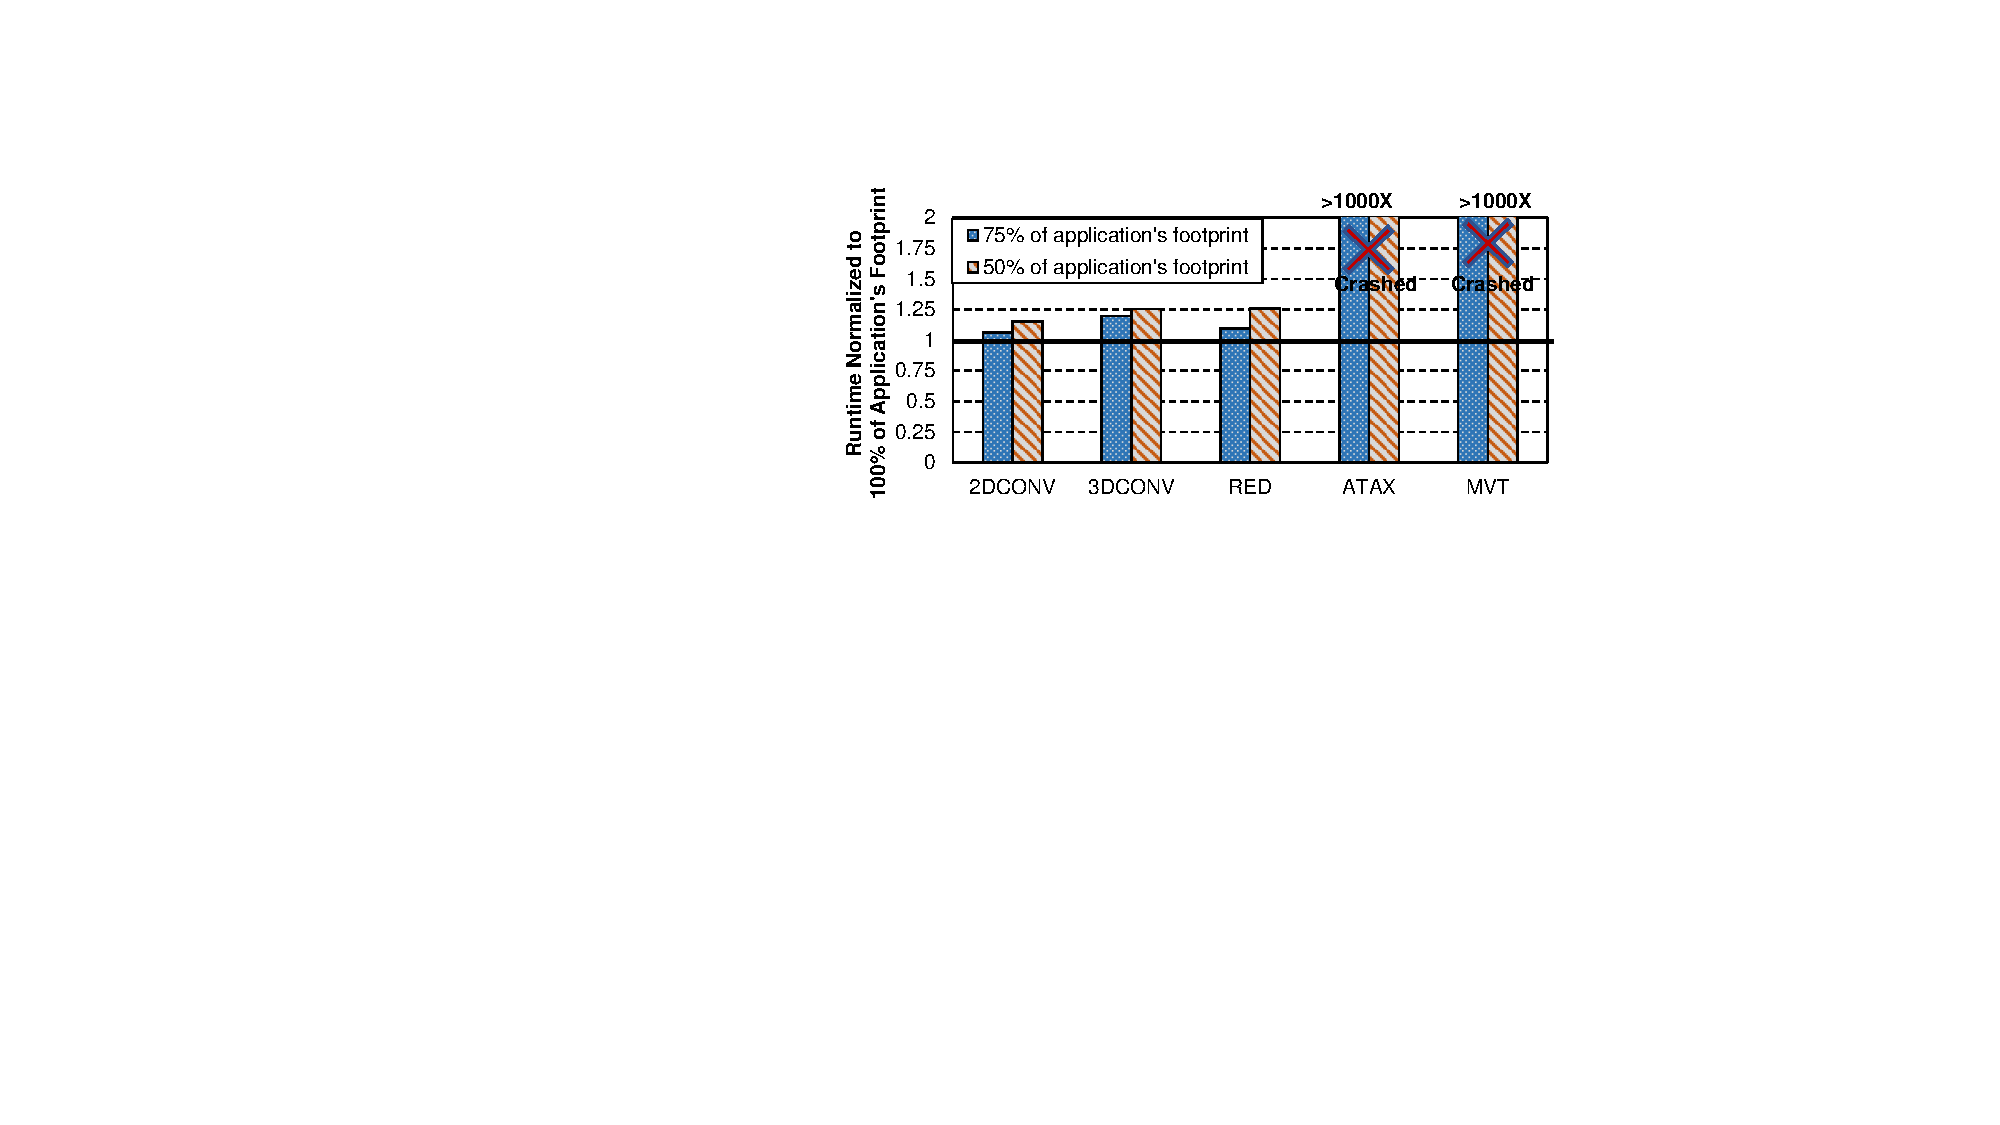
\includegraphics[width=5in]{/Figs_ETC/oversubscription_overhead_real}
  \caption{内存超额配置开销}
  \label{fig:oversubscription}
\end{figure}


图~\ref{fig:oversubscription}显示了内存超额配置下不同应用程序的性能损失。
本章观察了来自CUDA SDK~\upcite{cuda-sdk}和Polybench~\upcite{polybench}测试集的五个不同的GPGPU应用程序。
这些应用程序运行在一个拥有2GB可用内存的NVIDIA GTX 1060 GPU~\upcite{gtx1060}。
为模拟内存超额配置,我们手动地修改可用内存,使之分别是每个GPU内核函数所需内存容量的大约50\%和大约75\%。
从图~\ref{fig:oversubscription}中结果得出三点观察。
第一,所有的应用程序在内存超额配置的情况下均出现了显著地性能下降:内存超额配置率越高,性能下降的程度越大。
第二,2DCONV、3DCONV和RED三个应用程序性能平均下降了17\%。
我们发现这个性能损失是由于为新拷贝的数据页腾出空间而等待现有物理页的逐出所导致的。
这也是规则应用程序的内存超额配置开销的主要来源。
第三,当有效内存容量为ATAX和MVT的内核函数所需内存空间的75\%时,两个应用程序的性能分别下降了超过1000倍,即出现了内存抖动的现象,即数据页会不停在CPU和GPU内存之间来回迁移;
而当GPU的有效内存空间仅能满足应用程序所需内存空间的50\%时,内存抖动现象进一步恶化,该现象产生过多缺页中断,在严重内存超额配置的情况下直接导致系统宕机。


\section{设计空间探索:一种应用透明的框架}
\label{sec:etcexplore}

\textbf{先前避免内存超额配置的方法}。
之前有许多技术都可以用来管理内存超额配置。
增加存储容量是避免内存超额配置最有效的方法。
例如封装内的三维堆叠存储器High-Bandwidth Memory(HBM)~\upcite{hbm2,lee-taco2016}和Hybrid Memory Cube(HMC)~\upcite{hmc1,hmc2})已经被广泛应用到了NVIDIA P100~\upcite{pascal}和V100 GPU~\upcite{volta}、AMD Radeon R9系列GPU~\upcite{AMDVEGA}、以及谷歌的TPUv2~\upcite{Jouppi:2017:IPA:3079856.3080246,GoogleTPUv2}上。
然而,增加封装内的三维堆叠存储器的存储容量依然面临着三大主要挑战。
首先,堆叠的层数受到了半导体制造技术的限制;
其次,在硅中介层水平方向堆叠更多的存储器受到硅中介层引线复杂度和处理器引脚数目的限制~\upcite{loh2015interconnect};
第三,随着GPU应用程序数据集持续增长,应用程序开发者仍然需要考虑如何使用有限的存储容量~\upcite{kwon2018case, micro-memory-centric}。
除此之外,还有一些方法将任务划分并分配到多个GPU,或者将任务划分成更小的粒度,使得每个任务所需要处理的数据所占的存储空间小一点~\upcite{vast,gawande2018scaling}。
但是,这些方法都需要程序员花费很大的精力将一个复杂的大GPU任务分解,对程序员的要求非常高。
将任务分配到多GPU系统还会引入更多的GPU之间以及CPU和GPU之间的通信,这也将带来额外的开销。

\textbf{初始设计空间探索}。
为了缓解内存超额配置开销,我们尝试了多种不同的方案和策略进行设计空间探索。
这些策略的主要目标是降低缺页中断开销。
我们测试了不同的warp调度策略。
例如我们分别为发出缺页中断请求的warp和无缺页中断请求的warp给定不同的优先级。
非缺页中断请求的warp将拥有较高优先级,因此该warp已在内存中的数据能尽快被继续处理。
但是,我们发现这种warp调度策略并不能减少缺页中断,只是将集中的缺页中断请求分散。
最终,所有的线程都会在等待缺页中断处理的完成而停滞。
由此我们得出结论,虽然warp级别的调度策略是掩藏内存访问延迟的有效方法,但这还是难以掩藏缺页中断处理延迟,因为缺页中断处理的延迟比访存延迟大了多个数量级。

我们也实验测试了几种不同的页替换策略来强化局部性特征并将内存抖动最小化。
传统想法认为理想的LRU策略(Least Recently Used Policy)~\upcite{belady}是页替换策略可以达到的性能上限,然而LRU策略在GPU内存上实现太过昂贵,需要大量的查表和元数据存储开销。
基于时序的LRU策略(Age-based Least Recently Used Policy)则是一个更好的选择,该决策只需要一个列表存储每一个数据页从CPU内存移入GPU内存的时间,相对易于管理维护~\upcite{unifiedmemory2017,unifiedmemory2018}。
我们的实验显示,基于时序的LRU策略对于流访问模式的应用程序效果非常显著,这种访问模式的应用程序即为我们定义的具有强序列局部性的规则应用程序。
然而对于非规则应用程序,也就是随机访问模式的应用程序,基于时序的LRU策略并不奏效。
在这种应用程序中,我们观察到内存超额配置会引起严重的内存抖动。
因此,没有任何一种页替换策略能够有效减少内存抖动。

\textbf{设计目标}。
本章主要有三个设计目标。
第一,尽最大可能恢复内存超额配置下的程序性能到应用程序拥有足够的可用内存时的水平;
第二,设计的框架必须对应用程序透明,因为我们不希望程序员手动管理物理内存;
第三,本章的设计必须能够同时满足不同类型应用程序的不同需求。

\begin{figure}[htb]
\centering
\subfloat[规则应用程序]{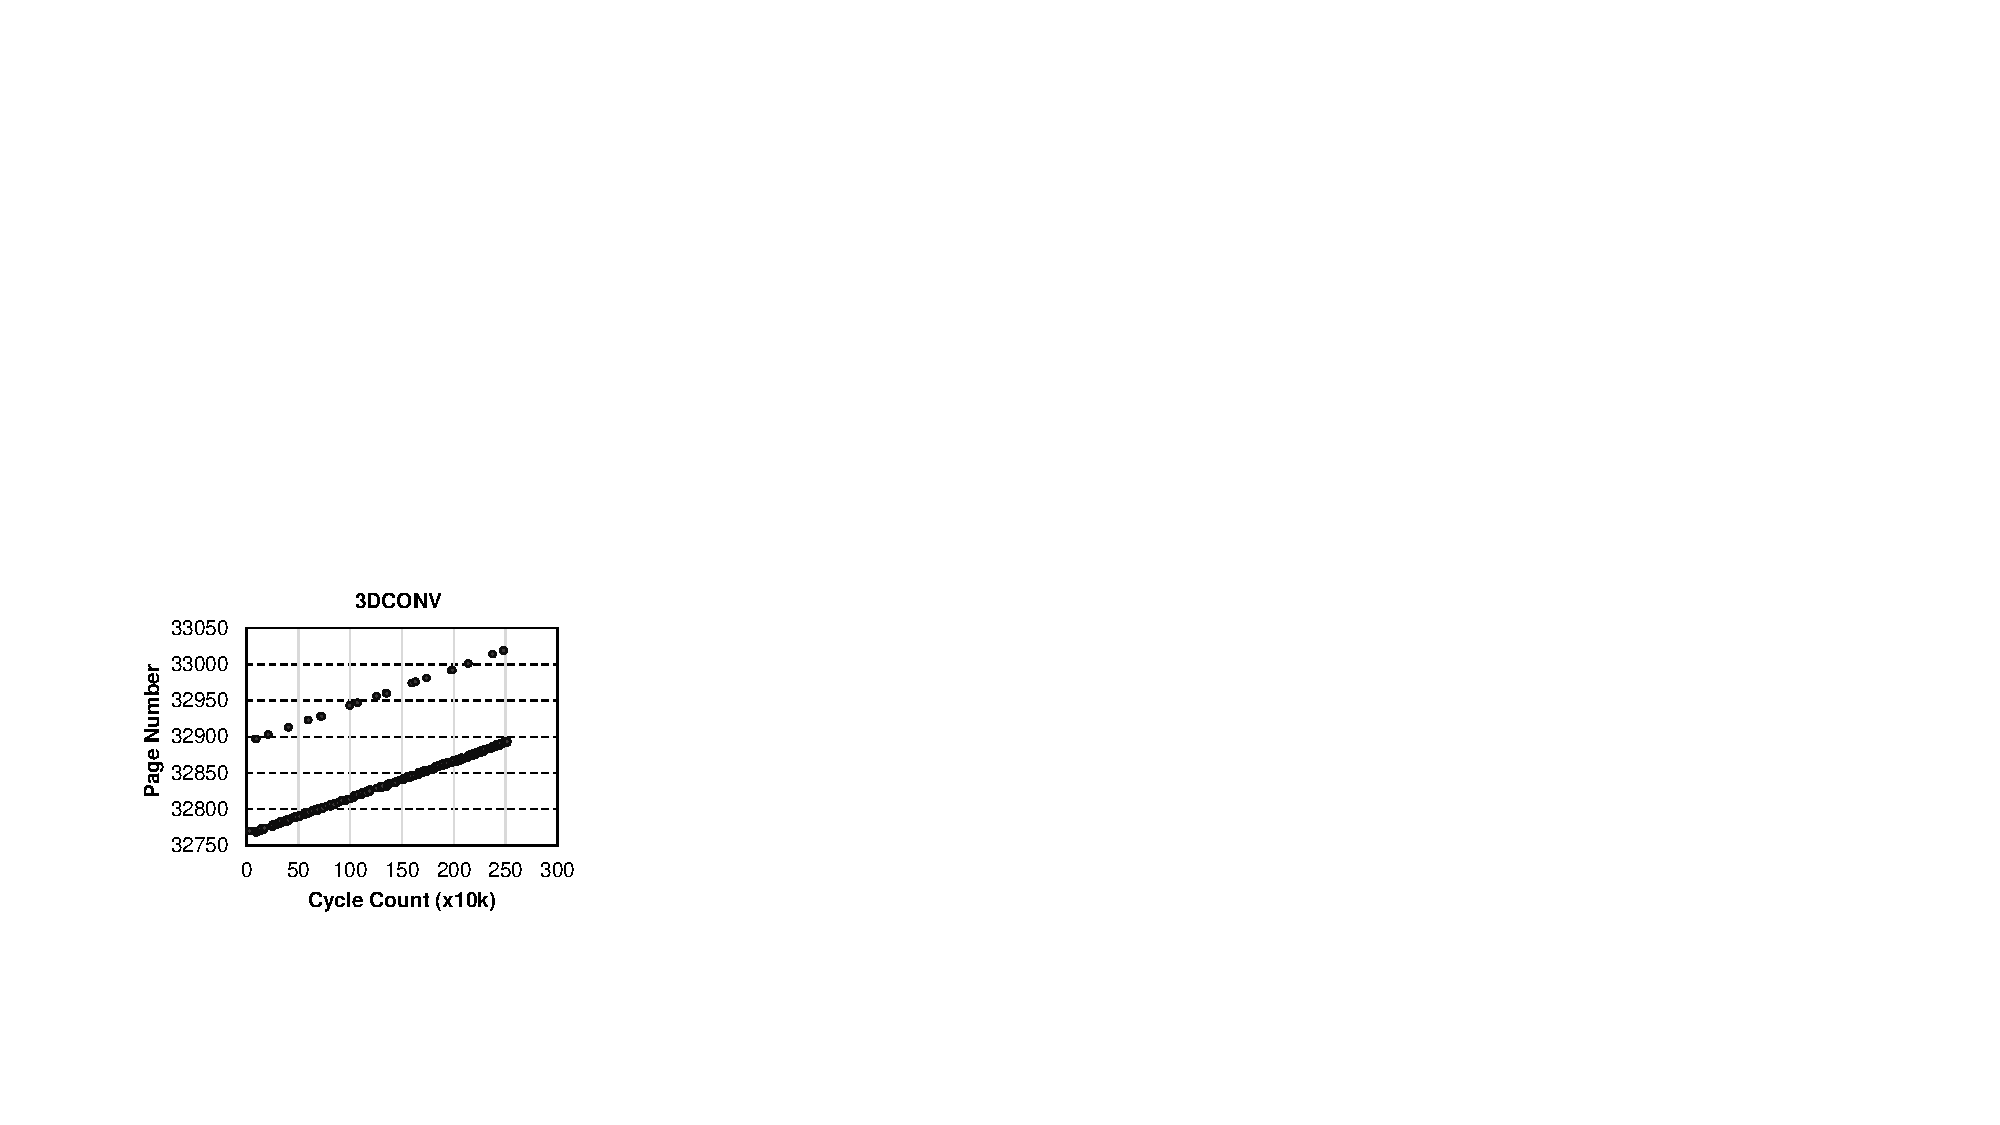
\includegraphics[width=.6\textwidth]{/Figs_ETC/Trace_3DCONV_1}} \qquad
\subfloat[非规则应用程序]{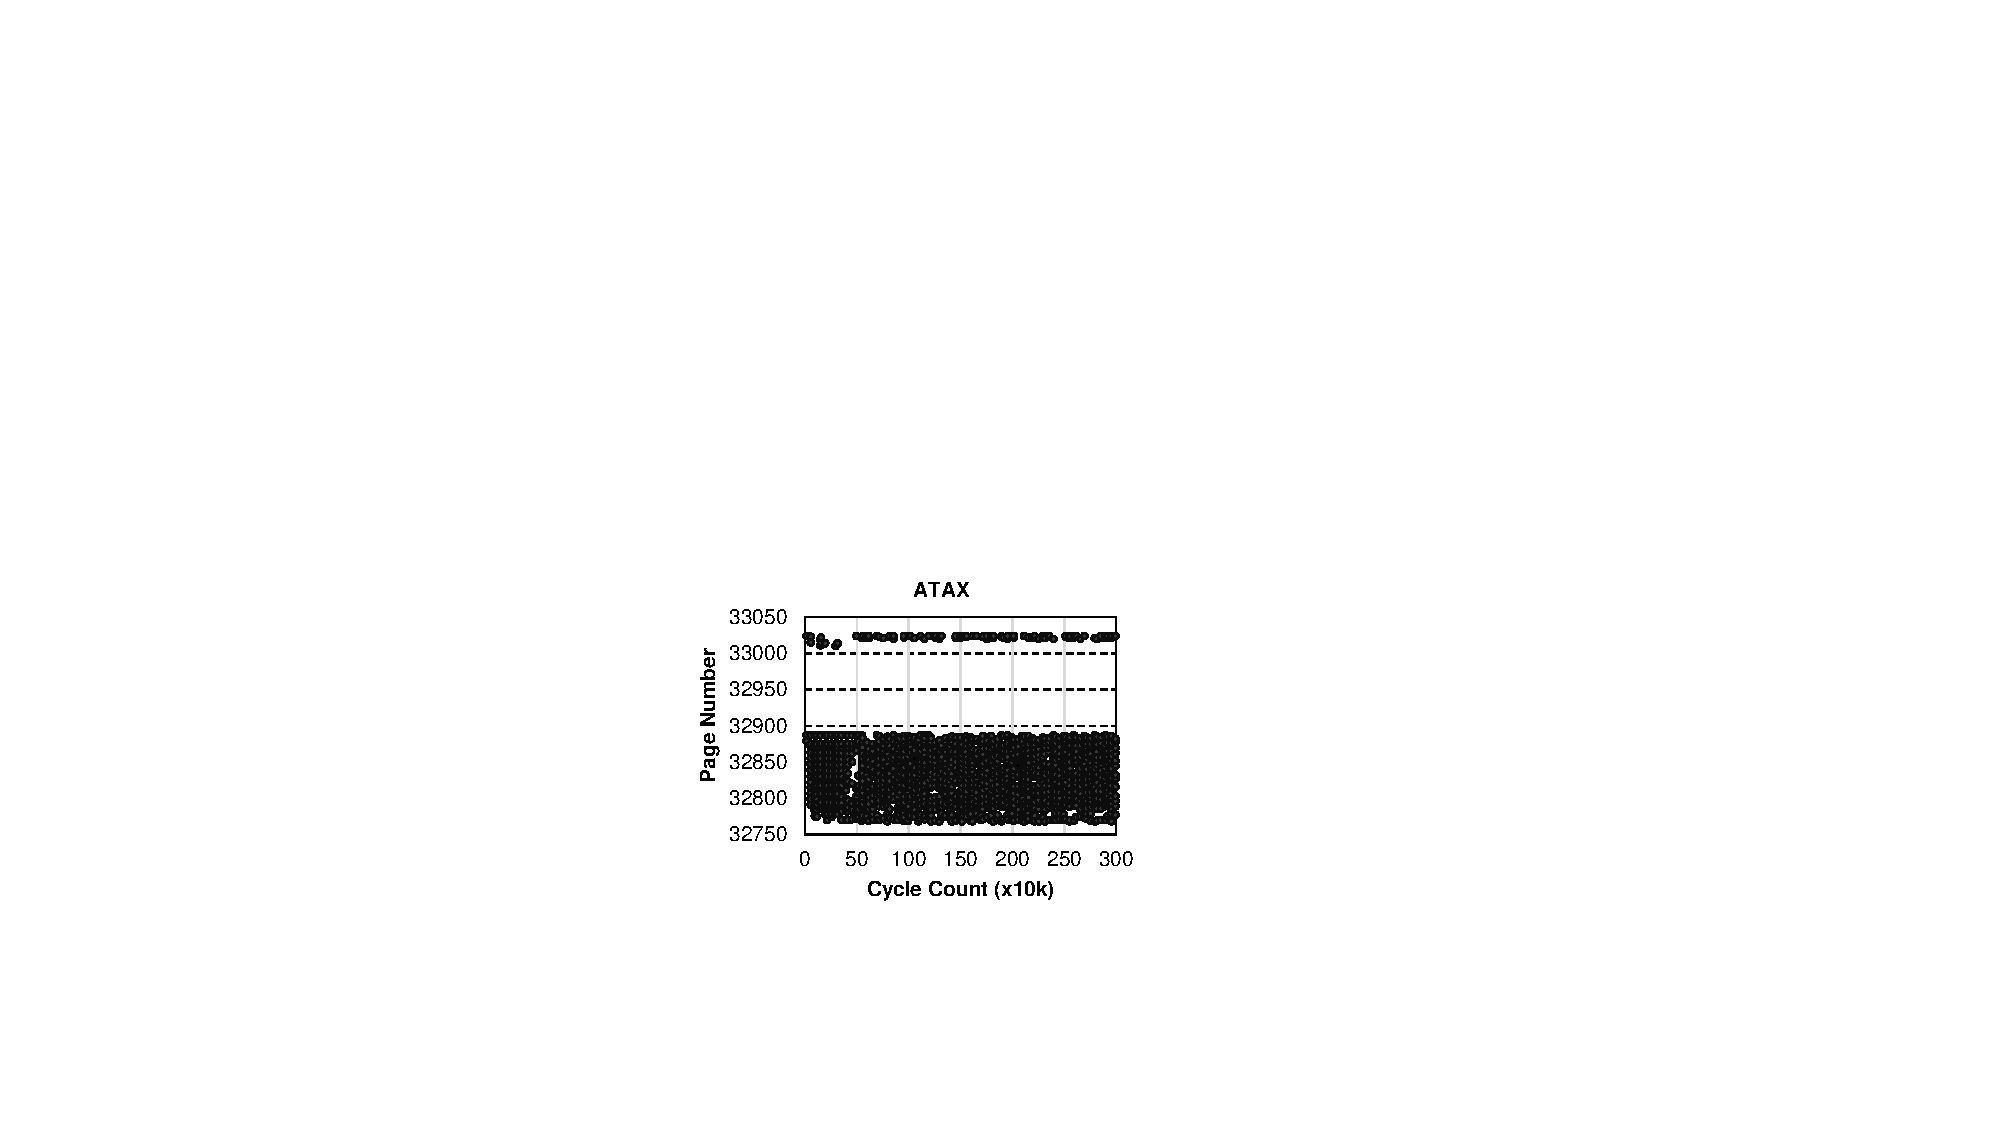
\includegraphics[width=.6\textwidth]{/Figs_ETC/Trace_ATAX_1}}  
\caption{数据页访问特性实例:(a)规则应用程序和(b)非规则应用程序}
\label{fig:Trace_1}
\end{figure}


\begin{figure}[htb]
\centering
\subfloat[规则应用程序]{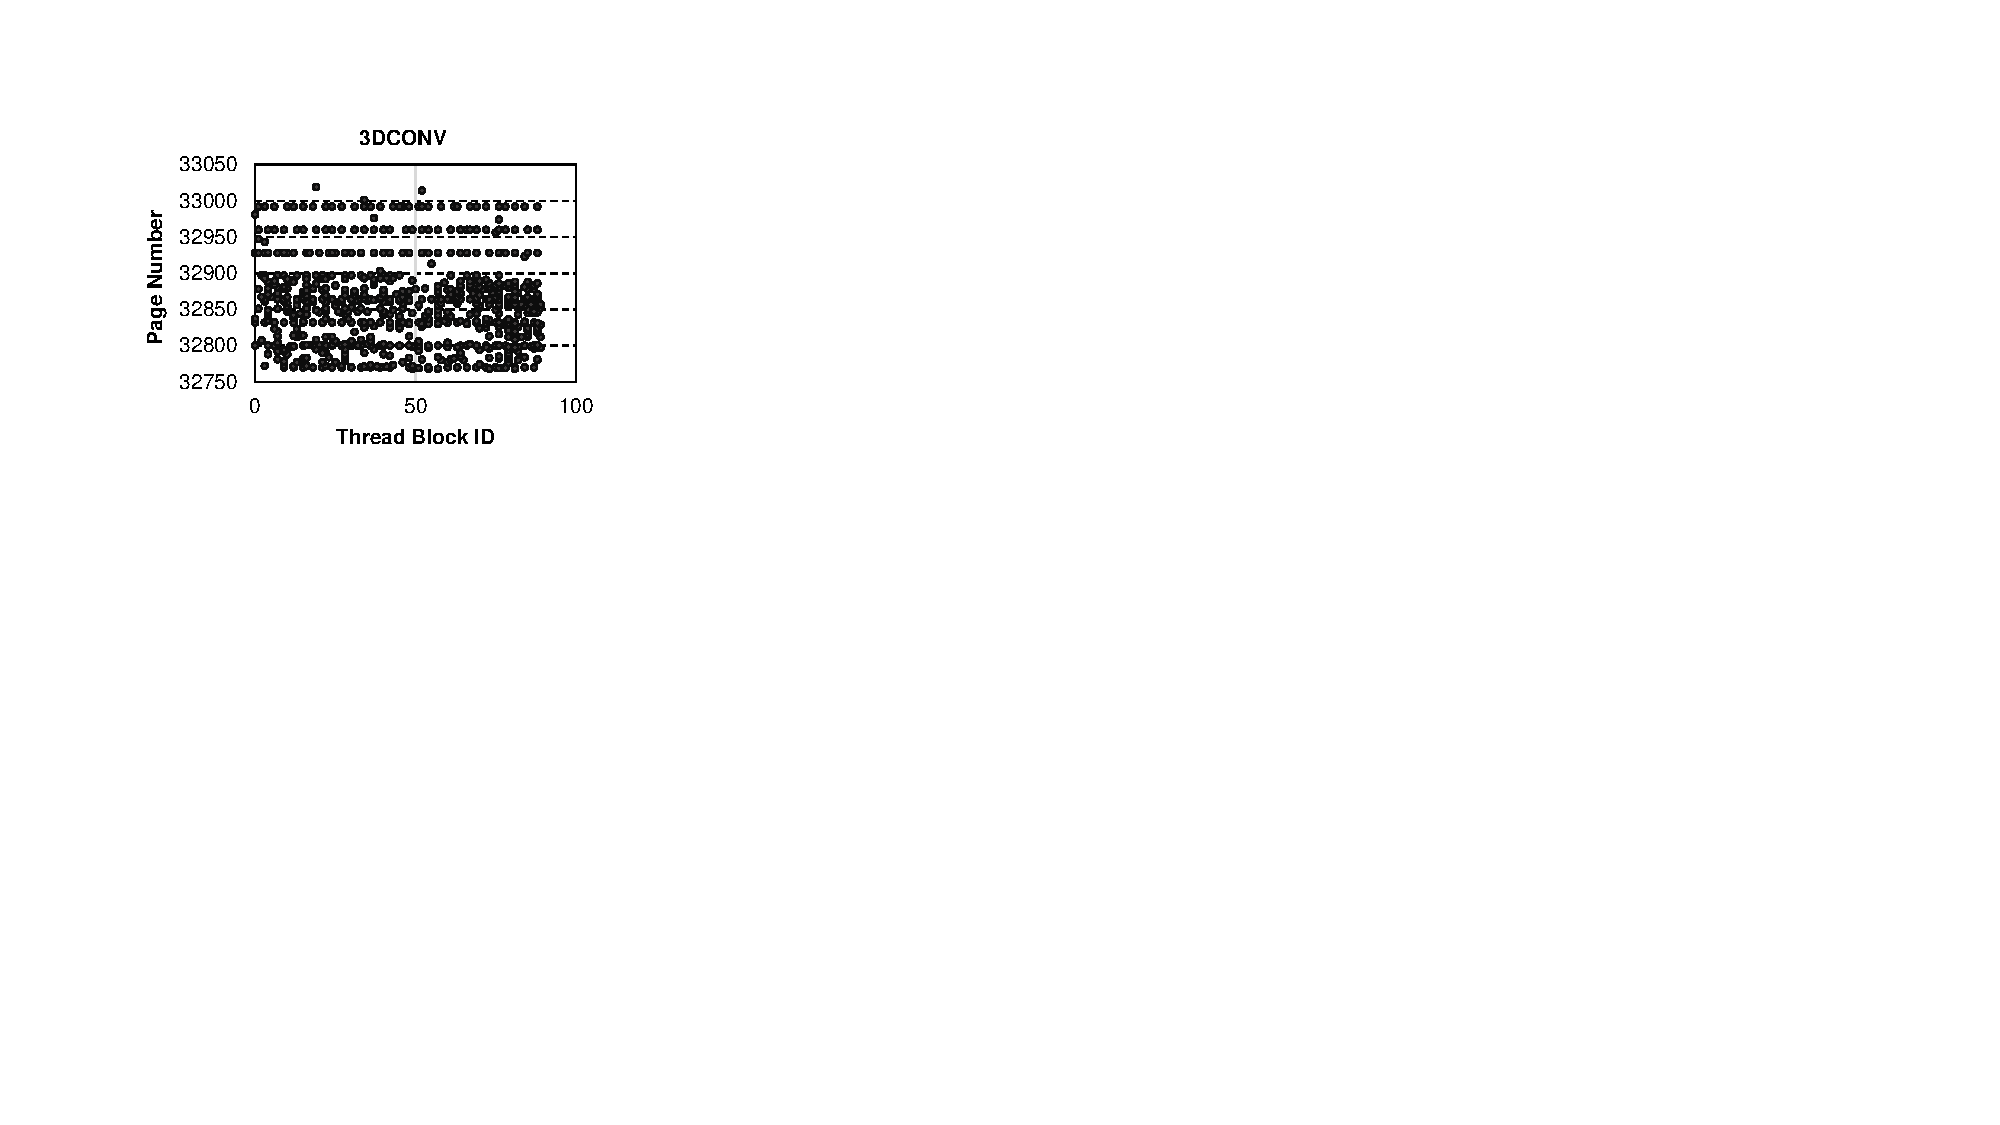
\includegraphics[width=.6\textwidth]{/Figs_ETC/Trace_3DCONV_2}} \qquad
\subfloat[非规则应用程序]{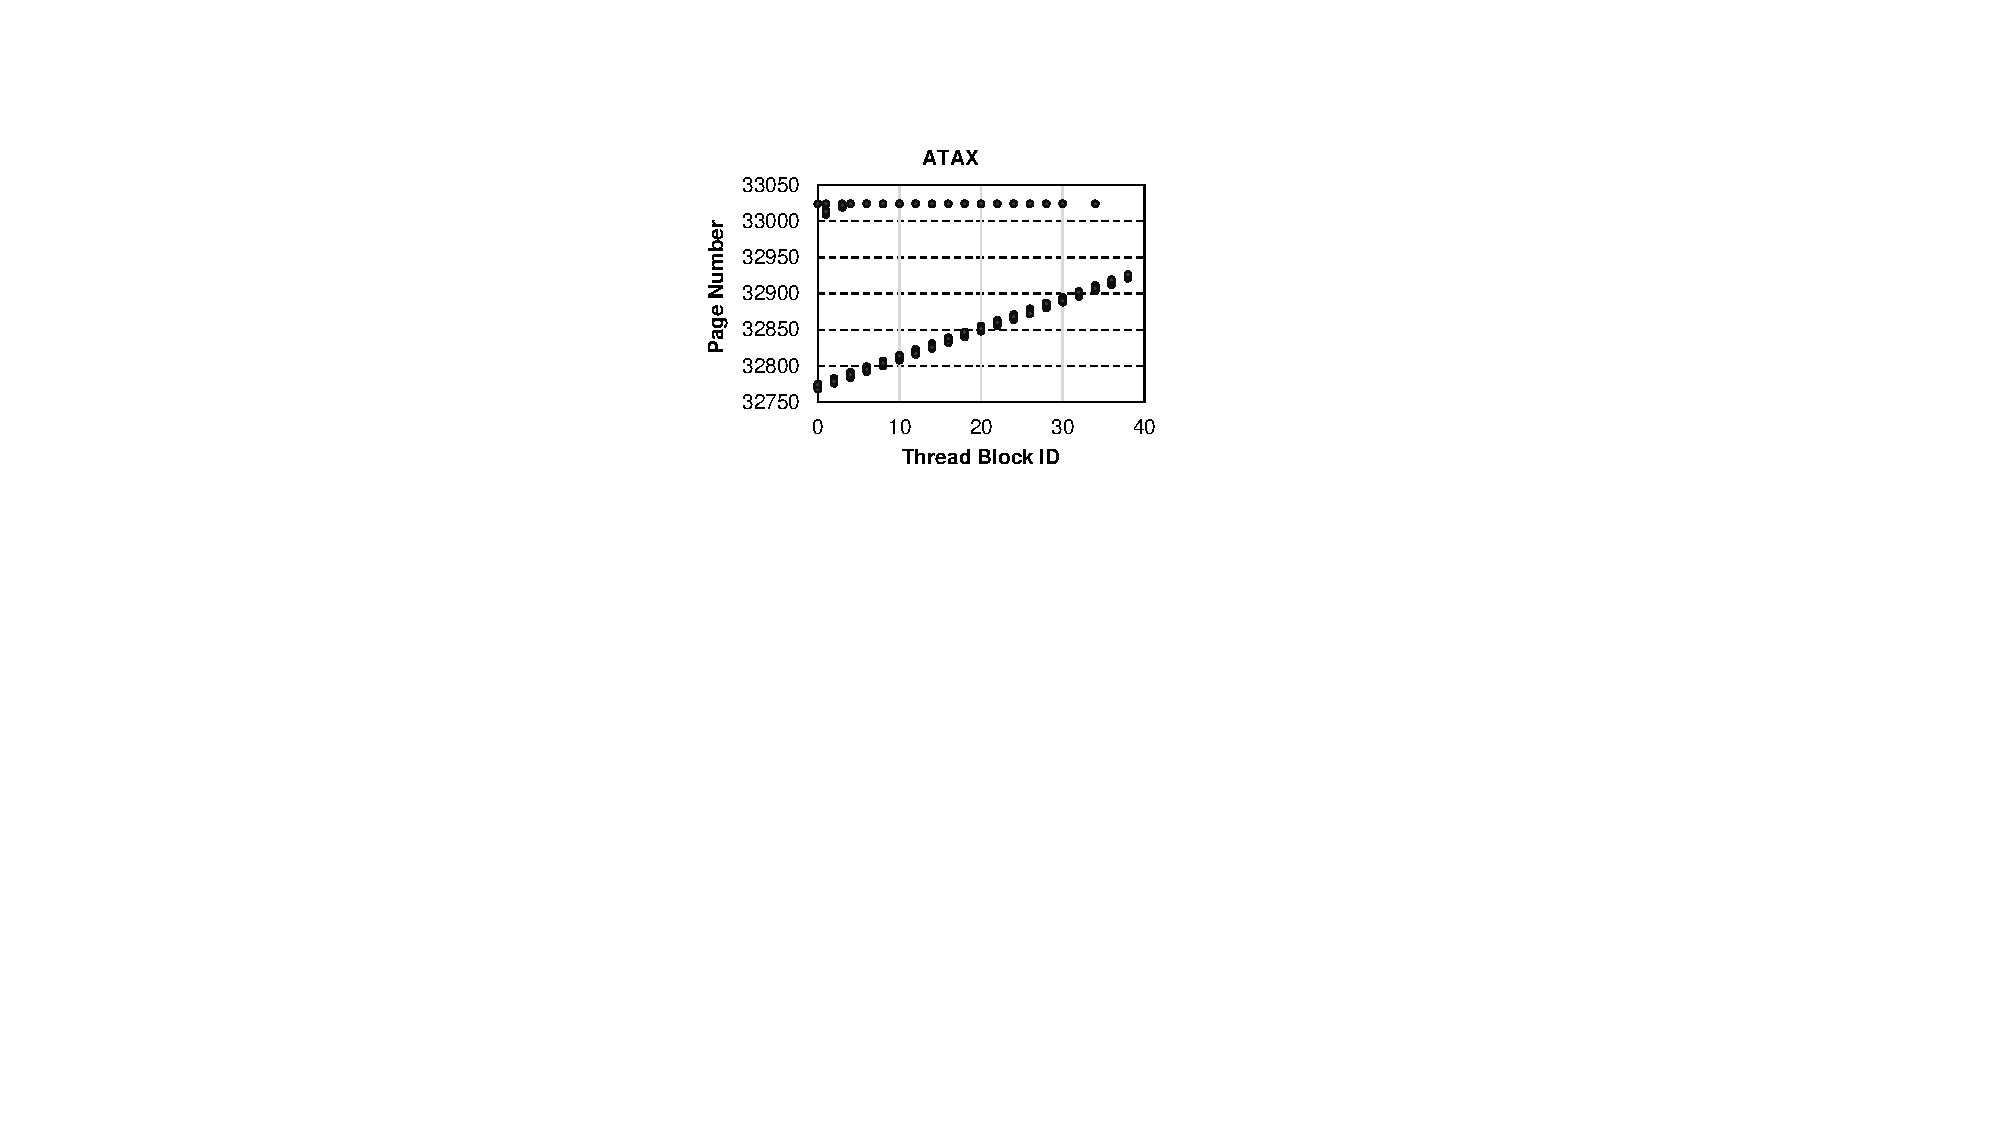
\includegraphics[width=.6\textwidth]{/Figs_ETC/Trace_ATAX_2}} 
\caption{线程块访问数据页关系实例:(a)规则应用程序(b)非规则应用程序}
\label{fig:Trace_2}
\end{figure}

\section{GPGPU应用程序的访存特性研究}
\label{sec:etcfeature}
设计一个有效的内存管理框架要求对应用程序访存特性有深入的分析理解,也就是应用程序的特性。
从这个角度出发,我们首先收集分析各种不同应用程序的访存trace,抽取其中最具有代表性的访问模式。
我们发现,应用程序一般可以被划分为规则访问模式和非规则访问模式。
图~\ref{fig:Trace_1}(a)-(b)显示了两个代表性应用程序,3DCONV和ATAX。
在线程块与数据页访问的关系中,3DCONV呈现出典型的流访问模式,而ATAX则呈现出一种相对随机的访问模式。
在任一时间点,3DCONV只访问非常少数量的数据页。
如图~\ref{fig:Trace_2}所示,几乎所有的线程块在一个时间点都在访问少量的几块数据页。
相反地,无论在任一时间点,ATAX都在同时访问大量的数据页。
如图~\ref{fig:Trace_2}(b)所示,ATAX的不同线程块访问的是不同的数据页。
我们还发现有许多应用程序都表现出和3DCONV类似的内存访问特征。
这一类应用程序的在线工作数据集相对较小,也就是说在一段时间内访问的数据量相对较小。
而像ATAX这一类非规则应用程序的在线工作数据集相对较大,因为每个线程都有可能访问一个新的不同的数据页。
这将导致在给定的时间内大量不同的数据页被访问。
此外,我们发现规则应用程序的访存是可以被预测的,如流访问模式,而非规则应用程序的访问模式是无法被预测的。


我们观察到对于规则应用程序,流访问模式的可预测性表现在被逐出的数据页通常都不会在一段时间后被重新请求,这很自然地避免了内存抖动现象。
但是,对于非规则的应用程序,预测访问模式非常困难,一旦在线工作数据集超出了有效的内存容量,任何被逐出的数据页都有可能短时间内再次被请求,导致内存抖动的发生。

\textbf{GPU内核函数间数据共享}。
另一种可能的情况是某些规则应用程序,不同的GPU内核函数访问并处理同一块数据。
如图~\ref{fig:LUD_trace}所示,在LUD中,每个内核函数的访存模式均为流访问模式且在线工作数据集相对较小。
但是,当一个应用程序的多个内核函数共享一块数据时,这块数据将被重复多次访问。
不同的内核函数之间存在同步栅栏,当数据大于物理内存的容量时,这块数据需要多次在CPU内存和GPU内存之间来回迁移,导致性能的大幅下降。

\begin{figure}[htbp] % use float package if you want it here
  \centering
  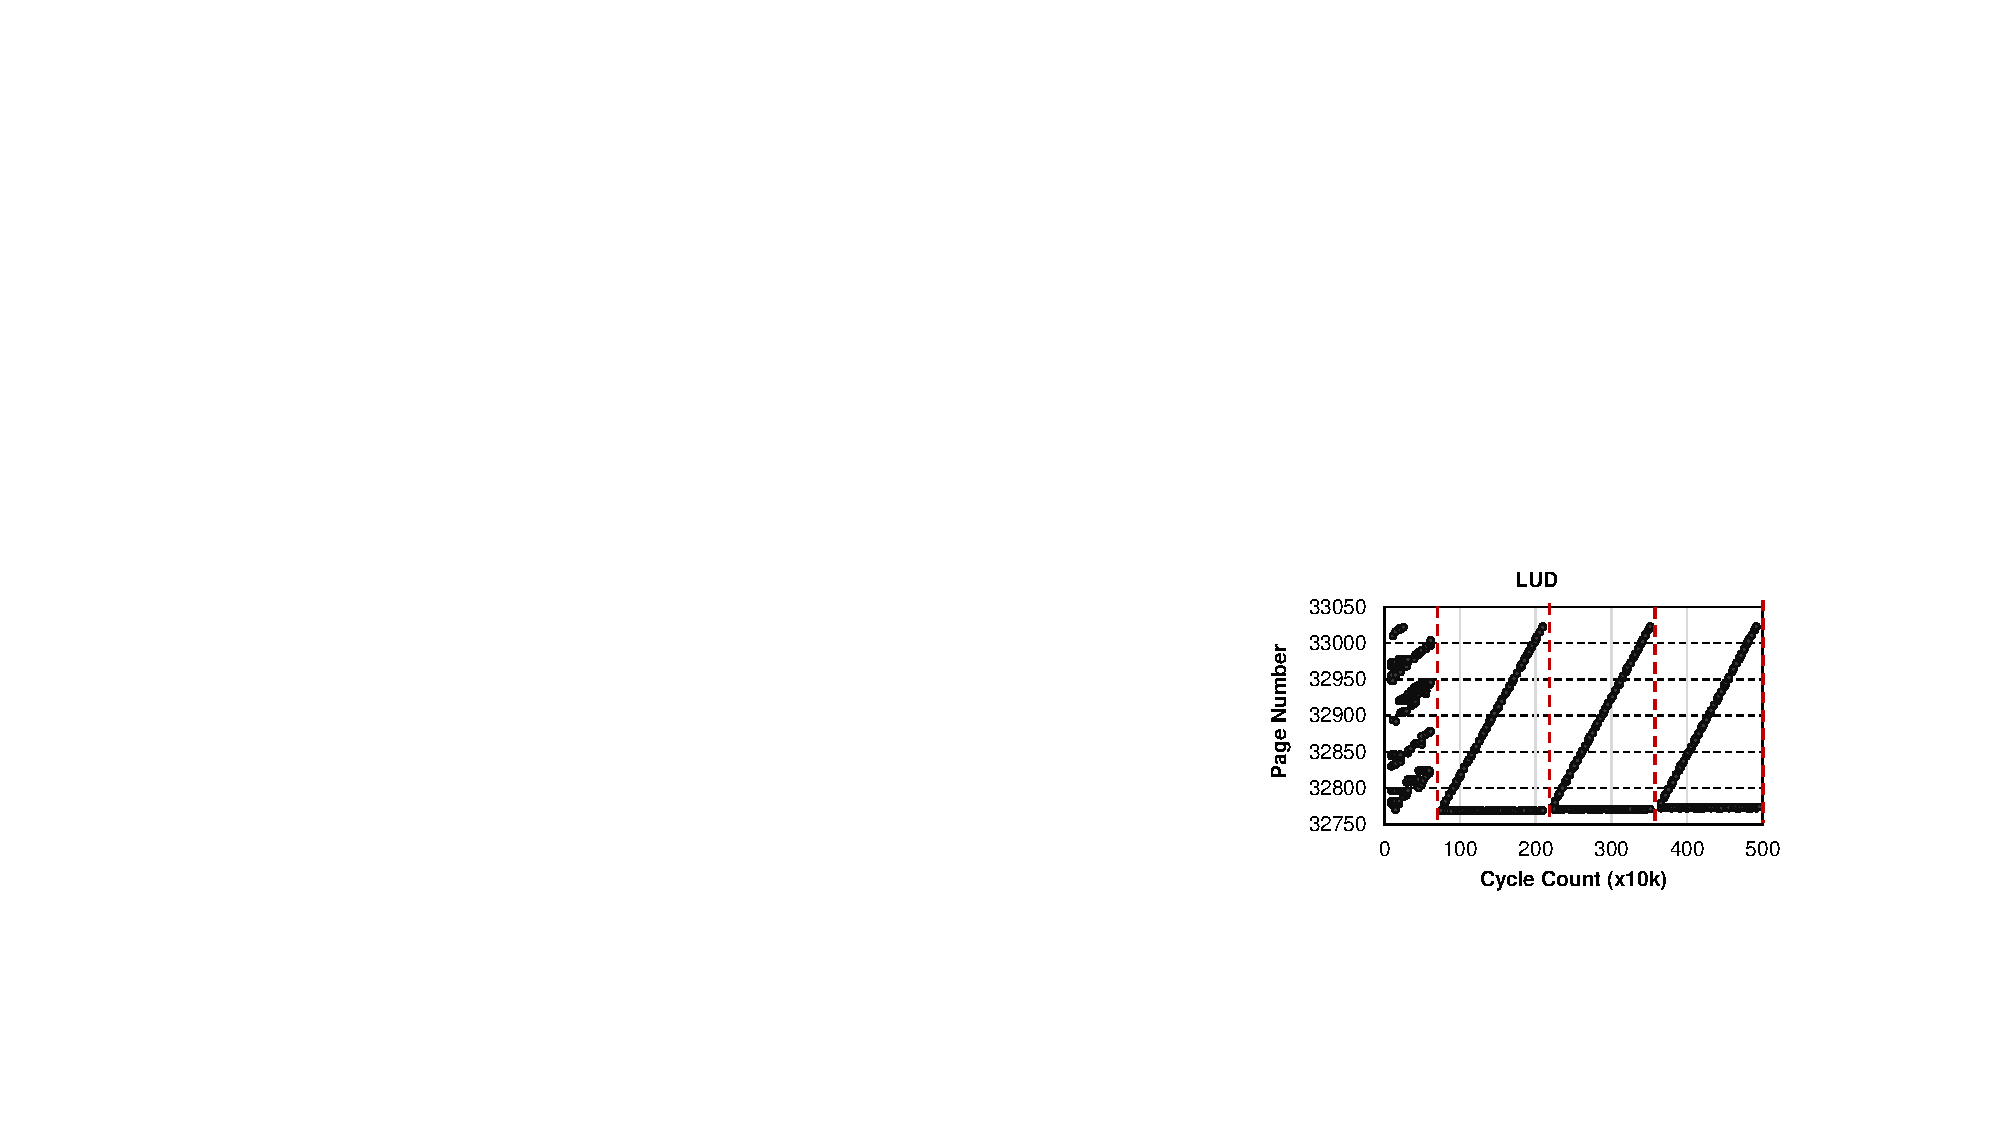
\includegraphics[width=.7\textwidth]{/Figs_ETC/LUD_trace}
  \caption{LUD数据页访问特性:数据共享的规则应用程序(多个内核函数访问同一块数据;虚线代表每个内核函数的结束时间点)}
  \label{fig:LUD_trace}
\end{figure}

基于以上发现,得出三点结论。
首先,数据页逐出等待时间是规则应用程序内存超额配置的最主要开销来源;
第二,内存抖动主导了非规则应用程序的内存超额配置的性能损失;
第三,数据共享引入了额外的数据迁移,导致更低的性能。
这三点结论将指导ETC框架的设计。

\section{ETC框架}
\label{sec:etcdesign}

ETC的核心思想是为不同类型的应用程序采用不同的内存管理技术以缓解内存超额配置的开销。
应用程序主要有三类:无数据共享的规则应用程序、数据共享的规则应用程序以及非规则应用程序。
基于这三类应用程序,ETC主要包含四个主要技术:\texttt{应用程序划分技术}、\texttt{主动数据页逐出技术}、\texttt{内存感知的并行度控制技术}、\texttt{以及内存容量压缩技术}。

一旦检测到内存超额配置,ETC首先对应用程序类别进行判定。
根据应用程序的类型,以及数据是否在多个内核函数之间共享,ETC框架会选择\texttt{主动数据页逐出}、\texttt{内存感知的并行度控制}以及\texttt{内存容量压缩技术}中的一种或多种进行内存超额配置下的性能优化。
对于规则应用程序,ETC会采用主动数据页逐出技术;
对于数据共享的规则应用程序,ETC在采用主动数据页逐出技术的同时还会采用内存容量压缩技术;
对于非规则应用程序,ETC会采用减少一部分运行的GPU核心来控制并行度,同时采用内存容量压缩技术来优化性能。

\subsection{应用程序划分}
\label{AC}

在ETC框架能够选择为哪种应用程序采用哪一种技术之前,它首先需要检测应用程序的类型,若为规则应用程序还需要检测是否存在不同内核函数之间的数据共享。
为检测每个GPU核心上运行的应用程序的类型,ETC框架采用访存合并系数作为判断指标,这种应用程序剖析的指标在GPU等单指令多线程体系结构的系统中被广泛使用~\upcite{jang2010exploiting,chatterjee2014managing}。
当来自于同一个warp的访存请求均访问的是同一个缓存行时,访存合并单元会将这些请求合并为一条访存请求以避免冗余访问,同时也可以减少带宽消耗。
对于规则应用程序,由于其访存局部性特征非常强,访存合并率也相应非常高~\upcite{cuda-sdk}。
但是对于非规则应用程序,由于其局部性特征不明显,访存请求更多地呈现出较低合并率~\upcite{polybench,parboil}。
基于这些观察,ETC框架在每个GPU核心的存取单元(LD/ST Unit)采用了一个计数器取样合并后的访存数。
如果合并后的访存数低于一定的阈值,则认为该GPU核心上运行的是规则应用程序,否则将该应用程序划分为非规则应用程序。

为检测多个内核函数间的数据共享,ETC依赖于在线编译技术。
当编译器检测到来自多个内核函数的访存指针指向接近的数据地址,则表明该应用程序的多个内核函数之间存在数据共享。
ETC标记共享统一数据指针的内核函数,并认为这些内核函数之间存在数据共享。

\subsection{主动数据页逐出技术}

主动数据页逐出的关键想法是预先地在GPU用完所有的物理内存空间之前就逐出旧数据页。
这将允许数据页逐出产生的数据迁移与缺页中断产生的数据迁移同时发生。
图~\ref{fig:Eviction_Overhead}给出了主动数据页逐出技术如何工作的例子。
如图~\ref{fig:Eviction_Overhead}(a),当数据页在GPU内存缺失时,失败的虚实地址转换会产生缺页中断,内存管理单元(Memory Management Unit, MMU)则会向CPU内存取该数据页。
如图~\ref{fig:Eviction_Overhead}(b)所示,如果应用程序用尽了物理内存,对新数据的访问需等到其他GPU内存中的数据页被逐出回CPU内存后才能执行。
在目前的商业GPU产品系统中,数据页逐出只能被缺页中断触发~\upcite{pascal,unifiedmemorycuda6}。

从CPU到GPU的内存迁移只能在GPU到CPU的数据页被逐出内存,数据迁移完成之后才能开始,如图~\ref{fig:Eviction_Overhead}(b)所示。
如图~\ref{fig:Eviction_Overhead}(c)所示,可以观察到通过重叠数据页逐出和缺页中断处理的延迟来掩藏逐出开销,实现降低内存超额配置开销的目的。

\begin{figure}[htbp] % use float package if you want it here
  \centering
  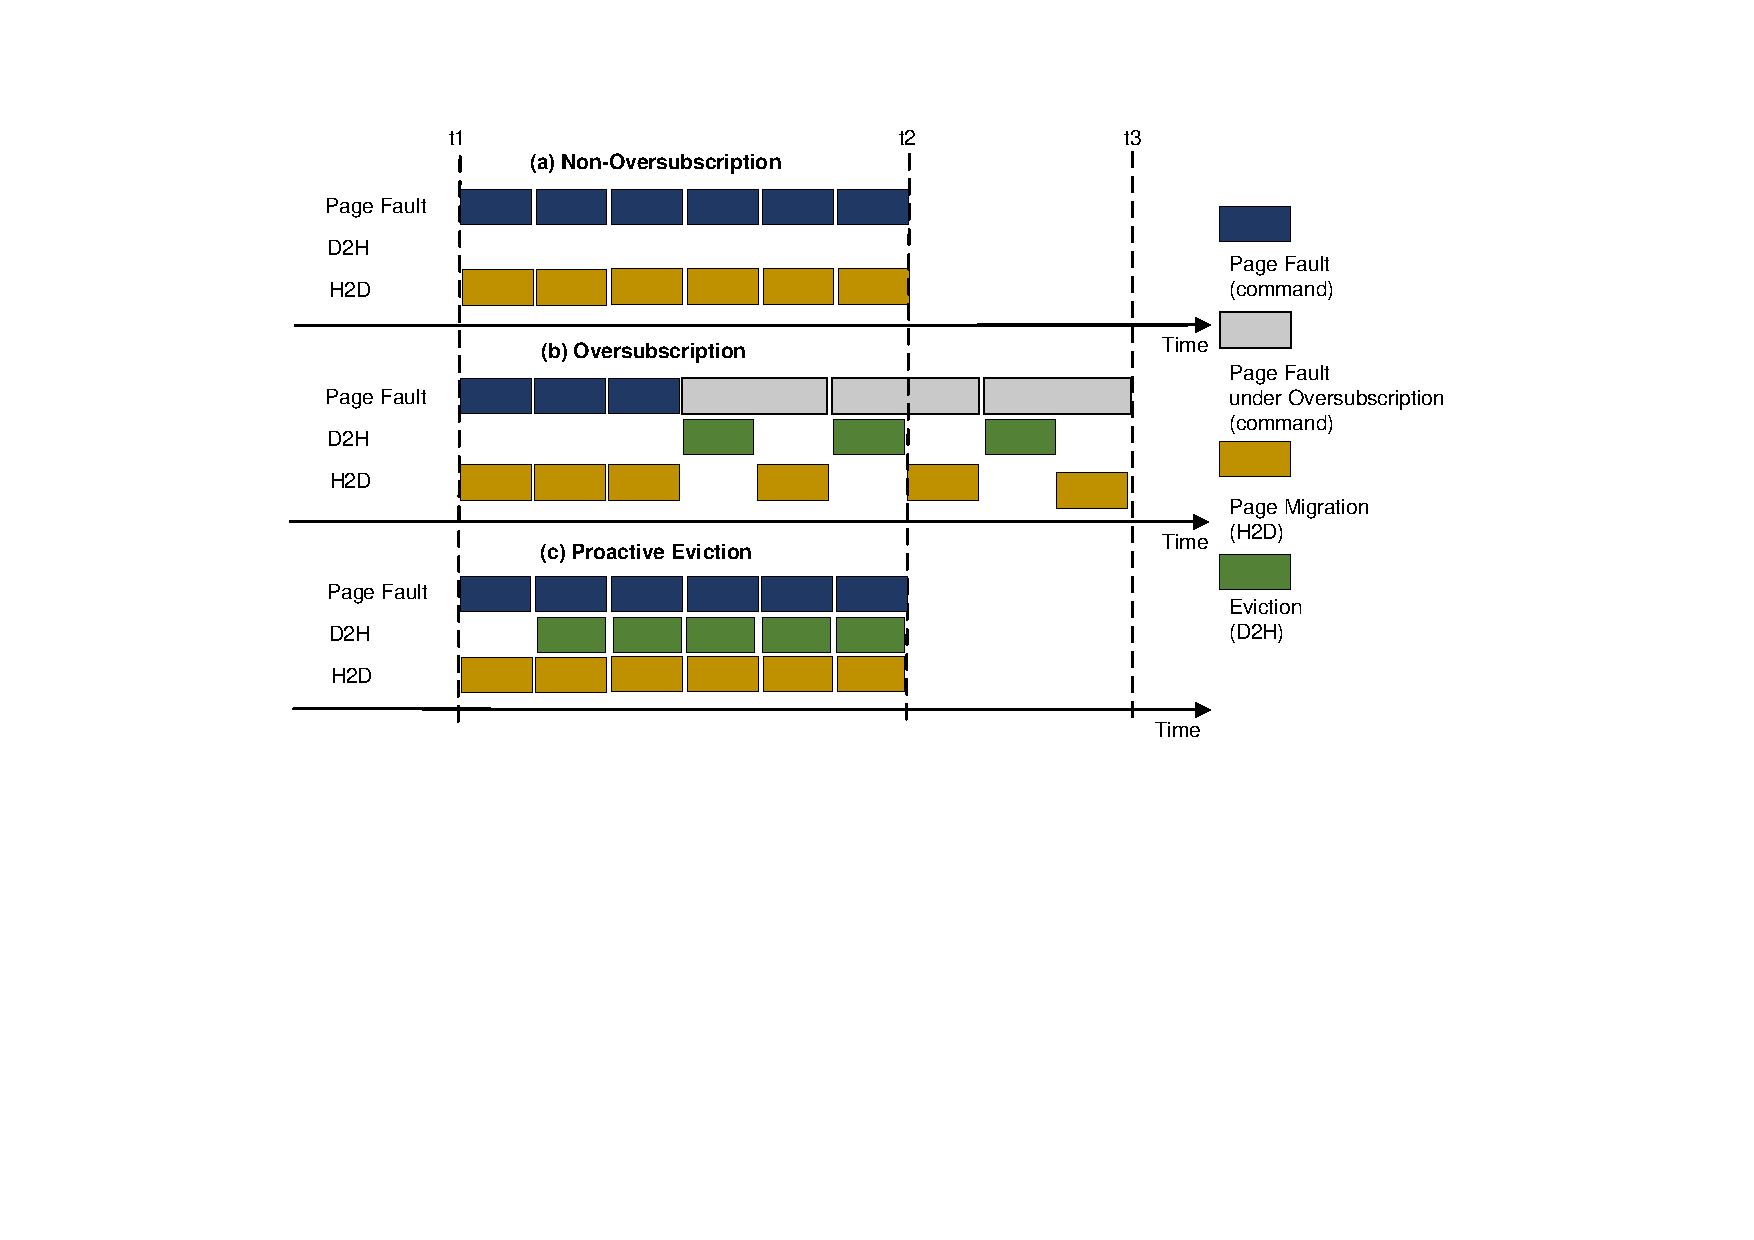
\includegraphics[width=\textwidth]{/Figs_ETC/Eviction_Overhead}
  \caption{主动数据页逐出技术}
  \label{fig:Eviction_Overhead}
\end{figure}


当前GPU支持双DMA引擎~\upcite{unifiedmemory2017, programmingguide,amd-fusion,AMDGCN},这使得缺页中断和数据页逐出产生的数据迁移理论上能够同时发生。
应用程序开发者可以通过手动操作并行预取和逐出操作来优化应用程序~\upcite{unifiedmemory2018}。
这种方法仍旧带给程序员巨大的负担,并且也违背了统一虚拟内存和实时按需取页的关键目标:减轻程序员负担。
为了自动的并行页逐出和缺页中断的数据迁移,我们修改GPU的驱动使得应用程序消耗完GPU所有物理内存之前就逐出页。
这样允许缺页中断的处理和页逐出的处理同时发生。

如何在最合适的时机进行主动页逐出是这个设计的重要挑战,也是需要我们解决的首要问题。
一方面,如果太早从GPU内存中逐出数据页会导致正在使用的数据页被逐出,该数据页很可能会被再次请求,带来额外的数据迁移开销;
另一方面,如果太晚逐出数据页很可能导致主动逐出失效。
另一个问题是,GPU驱动程序需要确定一次逐出操作涉及多少个数据页。
主动逐出过多的数据页也许可以减少GPU内存中不再使用的数据页,腾出更多的空间给新数据页。
但是,如果主动逐出过多的数据页会导致仍在使用的数据页被逐出,造成额外的开销。
我们开发出一种机制来平衡这个问题。

\textbf{避免过早的数据页逐出}。
为确定主动数据页逐出的正确时机,我们剖析在NVIDIA GTX 1060 GPU上运行的几个不同的GPGPU应用程序。
我们观察每个应用的内存访问轨迹,了解数据页从CPU迁移到GPU的数据量是如何增长的。
图~\ref{fig:footprint_rate}显示了五个GPGPU应用程序从CPU内存移动数据页到GPU内存的轨迹图。

\begin{figure}[htbp] % use float package if you want it here
  \centering
  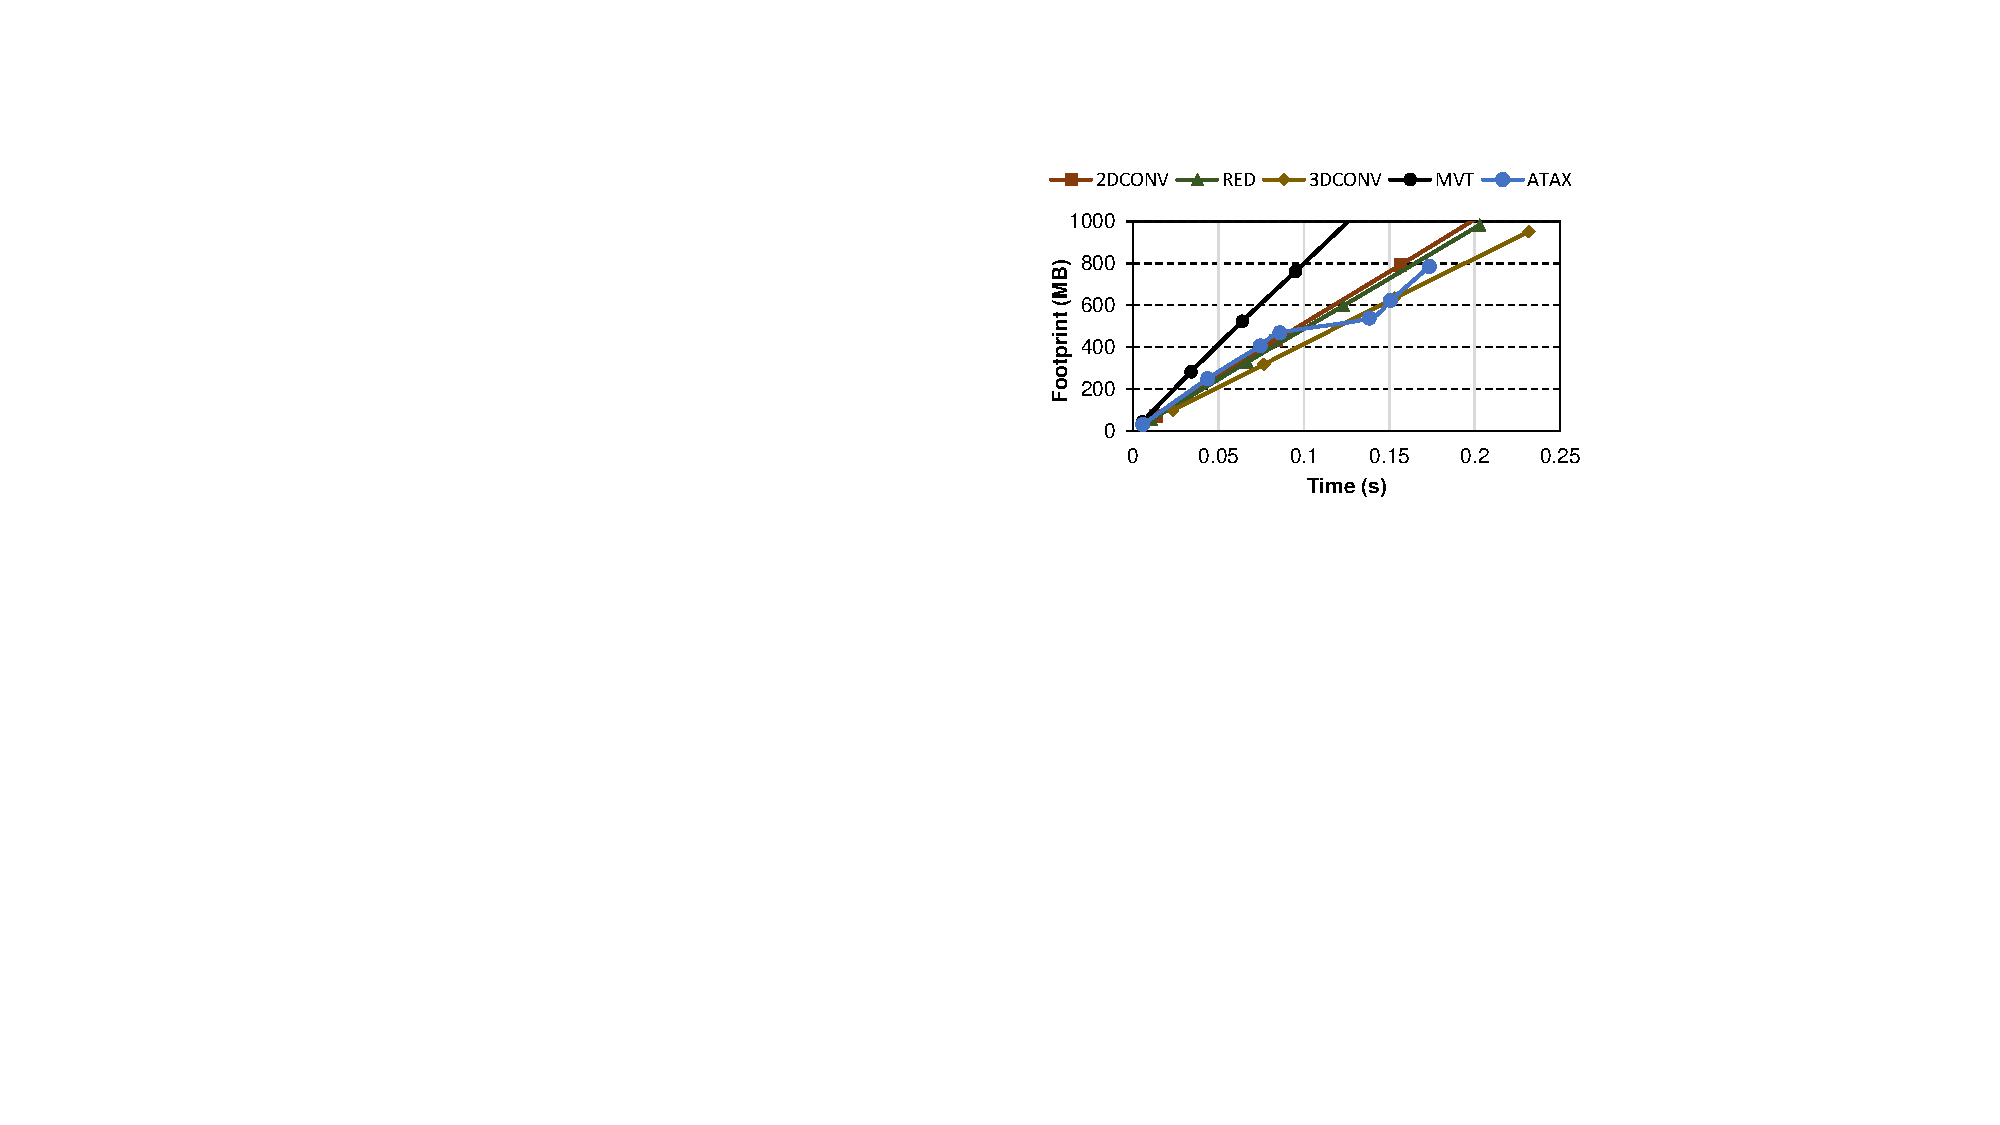
\includegraphics[width=.7\textwidth]{/Figs_ETC/footprint_rate}
  \caption{应用程序的内存占用随着时间的变化}
  \label{fig:footprint_rate}
\end{figure}


从数据中可以得出四点观察。
首先,内存占用大小是随着时间线性增长的;
其次,有可能出现多个增长的阶段(如ATAX的内存占用情况(图~\ref{fig:footprint_rate}中的蓝色点线)),但每个阶段内存占用的增长趋势仍然是线性的;
第三,GPU的单指令多线程工作模型显示,不同的warp执行相同的指令,但访问不同的数据。
当所有这些warp并行地执行,共享全局内存带宽,则内存占用会增加直到这个阶段所有的数据被取回。
这也解释了内存占用的增长为什么是线性的;
第四,缺页中断之间的时间间隔是相对固定的。
基于这些观察,GPU可以预测当一个缺页中断发生时,一系列的缺页中断在短时间内会相继稳定发生。
我们也可以触发多个数据页逐出请求,来为新需要的数据页腾出更多的空间。

\textbf{避免过晚的数据页逐出}。
我们发现CPU内存到GPU内存的数据传输速度并不总是和GPU内存到CPU内存的数据传输速度相同。
通过在NVIDIA GTX 1060 GPU的测试,我们发现从GPU内存到CPU内存的传输速度要明显快于CPU内存到GPU内存的传输速度。
因此,传输同样数量的数据页,从GPU内存传输回CPU内存的速度相对于从CPU内存传输到GPU内存速度稍快。
基于这些发现,我们可以在发生缺页中断的同时开始页逐出避免过晚地逐出页。

非规则应用程序在短时间内访问大量的数据页面。
因此,主动数据页逐出技术在非规则应用程序上使用将变得非常低效。
我们发现潜在地缺点是主动逐出数据页技术很可能会加剧非规则应用程序的内存抖动现象。

\textbf{实现方案}。
为了实现主动数据页逐出,ETC框架修改GPU runtime中的虚拟内存管理单元,增加主动数据页逐出单元(PEU)。
当缺页中断发生时,PEU中断GPU驱动,使之移动缺失的数据页到GPU内存。
当GPU驱动可成功分配一块新数据页到GPU内存时,PEU首先开始检查应用程序划分逻辑。
然后,PEU检查内存分配空间大小,并与有效内存容量比较来预测是否内存超额配置。
主动数据页逐出单元在以下情况被同时满足时会被触发:1.内存超额配置; 2.有效内存小于一定的阈值(经验设置小于2MB);3.应用程序被划分为规则应用程序。


\subsection{内存感知的并行度控制}

如~\ref{background}讨论的,数据页层次的内存抖动会显著降低非规则GPGPU应用程序的性能。
如图~\ref{fig:Trace_1}(b)和~\ref{fig:Trace_2}(b)所示,通常情况下,非规则应用程序的一个数据页仅被少量的线程块访问,不同的线程块访问的数据页也不一样。
当GPU许多非规则应用程序的线程块同时执行时,在线工作数据集快速增长,产生严重的内存抖动。
这是传统页替换策略无法解决的。
为了避免内存抖动,我们的核心思想是限制同时访问内存和取数据页的数量。
从这个角度出发,我们设计了内存感知的并行度控制技术,其目标是通过限制并行的线程数量,来减少非规则应用程序的有效在线工作数据集。
GPU并行度控制技术可以有两种实现方式,一种是线程块并行度控制,另一种是GPU核心(SM)并行度控制。
线程块并行度控制降低每个GPU核心内部的线程块的并行度。
而GPU核心并行度控制则降低每个GPU中计算核心的并行度。
我们实验了这两种方法并发现线程块并行度控制方法引入了相对过长的时间来达到最少的内存抖动。
与线程块并行度控制相比,计算核心并行度控制相对更快限制并行度使之达到最合适的在线工作数据集大小。
因此,ETC采用了GPU计算核心并行度控制的方法来减少GPU中的内存抖动现象。

\textbf{实现方案}。
当非规则应用程序被检测到且发现内存超额配置时,ETC会触发我们基于阶段的计算核心并行度控制技术。
当并行度控制被触发,ETC框架首先通过暂停一半GPU核心的取指功能,已经在流水线中的指令将继续执行直到完成。
在这个初始阶段,ETC框架很可能停掉了过多的GPU核心,导致较低的利用率;
另一种情况是停掉的GPU核心数量太少,导致内存抖动现象仍然存在。
因此在初始阶段之后,ETC框架需要基于观察到的内存利用率自适应地动态调整可执行的GPU核心数量。
如图~\ref{fig:sm_throttling}所示,内存感知的并行度控制将GPU的执行划分为两个阶段:\texttt{检测阶段}和\text{执行阶段}。
在检测阶段,ETC首先检测是否出现了逐出请求或缺页中断请求来判断初始阶段ETC的计算核心并行度控制是否过度。
如果一个缺页中断请求被检测,或者检测阶段的运行时间结束,检测阶段将停止。
一旦检测阶段停止,执行阶段开始,内存感知的并行性控制技术完成自适应调整,不再调整可运行的计算核心的数量,继续执行直到本阶段结束。

\begin{figure}[htbp] % use float package if you want it here
  \centering
  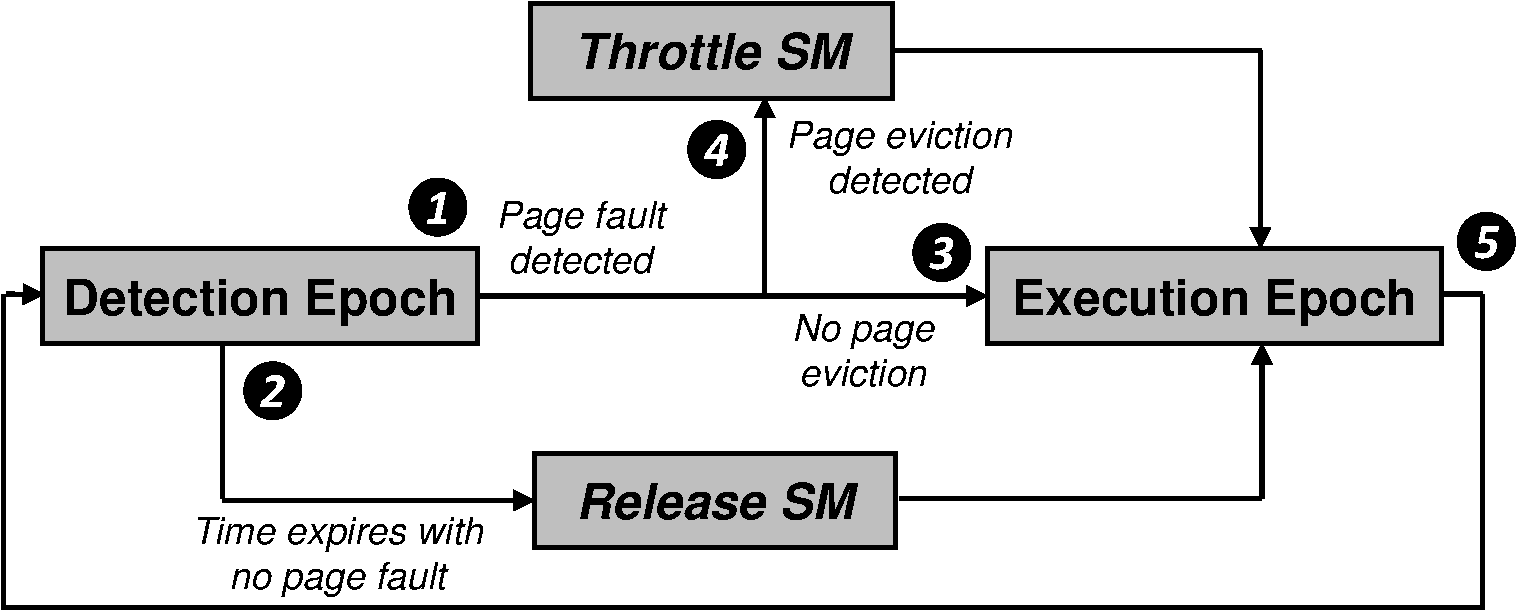
\includegraphics[width=\textwidth]{/Figs_ETC/sm_throttling}
  \caption{ETC的内存感知的并行度控制策略)}
  \label{fig:sm_throttling}
\end{figure}

如果检测阶段的结束仅是因为检测阶段的时间完成,并没有发生缺页中断。
这说明当前的有效内存容量是足够当前的数据集的。
GPU还能够同时执行更多的线程,以更加高的内存利用率运行而无内存抖动存在。
在这种情况下,ETC框架将重新开始执行一个被暂停的计算核心。
为完成这一操作,ETC使上一个被停止取指的计算核心重新开始取指来实现GPU计算核心开启。

如果检测阶段的结束是因为一个缺页中断且无数据页逐出发生,这说明GPU依然有足够的有效内存空间。

如果检测阶段的结束时因为一个缺页中断,且发生至少一次数据页逐出,这表明GPU的内存容量已无法满足应用程序的在线工作数据集。
ETC框架需要限制更多GPU核心的执行,以减少在线工作数据集,使得内存容量足以容纳现有的工作数据集。
在这种情况,只要缺页中断处理完成,ETC将停止产生该缺页中断的GPU核心的取指功能,暂停其运行。
因为这个GPU核心最有可能是刚开始执行处理数据。

在每次调整之后,GPU会不受打扰地执行一段时间。
当所有可运行的GPU核心执行完执行阶段的时间后,GPU重新回到检测阶段,再次检测并调整可运行的GPU核心的数量。

通过内存感知的并行度控制方法,非规则应用程序的并行度被调整到在线工作数据集大小能完整地在内存中运行的状态。
虽然并行度控制技术在一定程度上降低了线程级的并行度,我们发现它能显著减少CPU内存和GPU内存之间的数据迁移,并且显著恢复因为内存超额配置造成的性能下降。
此外,这种并行度下降产生的性能损失,也可以通过结合容量压缩方法来挽回。这将在~\ref{compress}中具体介绍。

\subsection{内存容量压缩}
\label{compress}
通过之前的介绍可以知道,在内存超额配置的情况下,主动数据页逐出技术可以有效提高规则应用程序的性能,
而内存感知的并行度控制技术可以提升非规则应用程序的性能,但依然可能出现以上两种方法独立工作并不能提供足够性能的情况。
首先,ETC的主动数据页逐出技术可以掩藏数据页逐出延迟,但是在多个内核函数数据共享的情况下,不能减少CPU内存和GPU内存之间数据页迁移的次数;
第二,ETC的内存感知的并行度控制技术虽然对避免非规则应用程序的内存抖动情况非常有效,但它会带来线程级并行度下降的问题。

为了进一步降低内存超额配置的开销,我们的目标是提高内存的有效物理容量。
从这个角度出发,我们开发了一种内存容量压缩技术。
ETC内存容量压缩技术的核心想法是,根据应用程序的类型,选择性地使用内存容量压缩来提升性能。
以前已经有好几种主存压缩技术被提出~\upcite{lcp-micro13,ekman-isca05,rhu2018compressing,caba,kim2016bit},他们都能有效提高内存容量。
在本章中,我们采用了线性压缩数据页技术(Linear Compressed Page,LCP)~\upcite{lcp-micro13}来压缩GPU内存中的数据。

LCP内存压缩框架是一种低延迟的内存容量压缩框架。
之前在CPU的应用已显示其在提升主存容量方面非常有效。
我们发现LCP在GPU中性能会有严重影响,因为它需要额外的一次访存来获取存储在主存中的压缩相关元数据。
如图~\ref{fig:data_compression_overhead}所示,额外的一次LCP压缩框架元数据访问可以导致额外的带宽需求。
实验显示在无内存超额配置的情况下,这些应用程序在GPU的性能平均下降了13\%。




\begin{figure}[htbp] % use float package if you want it here
  \centering
  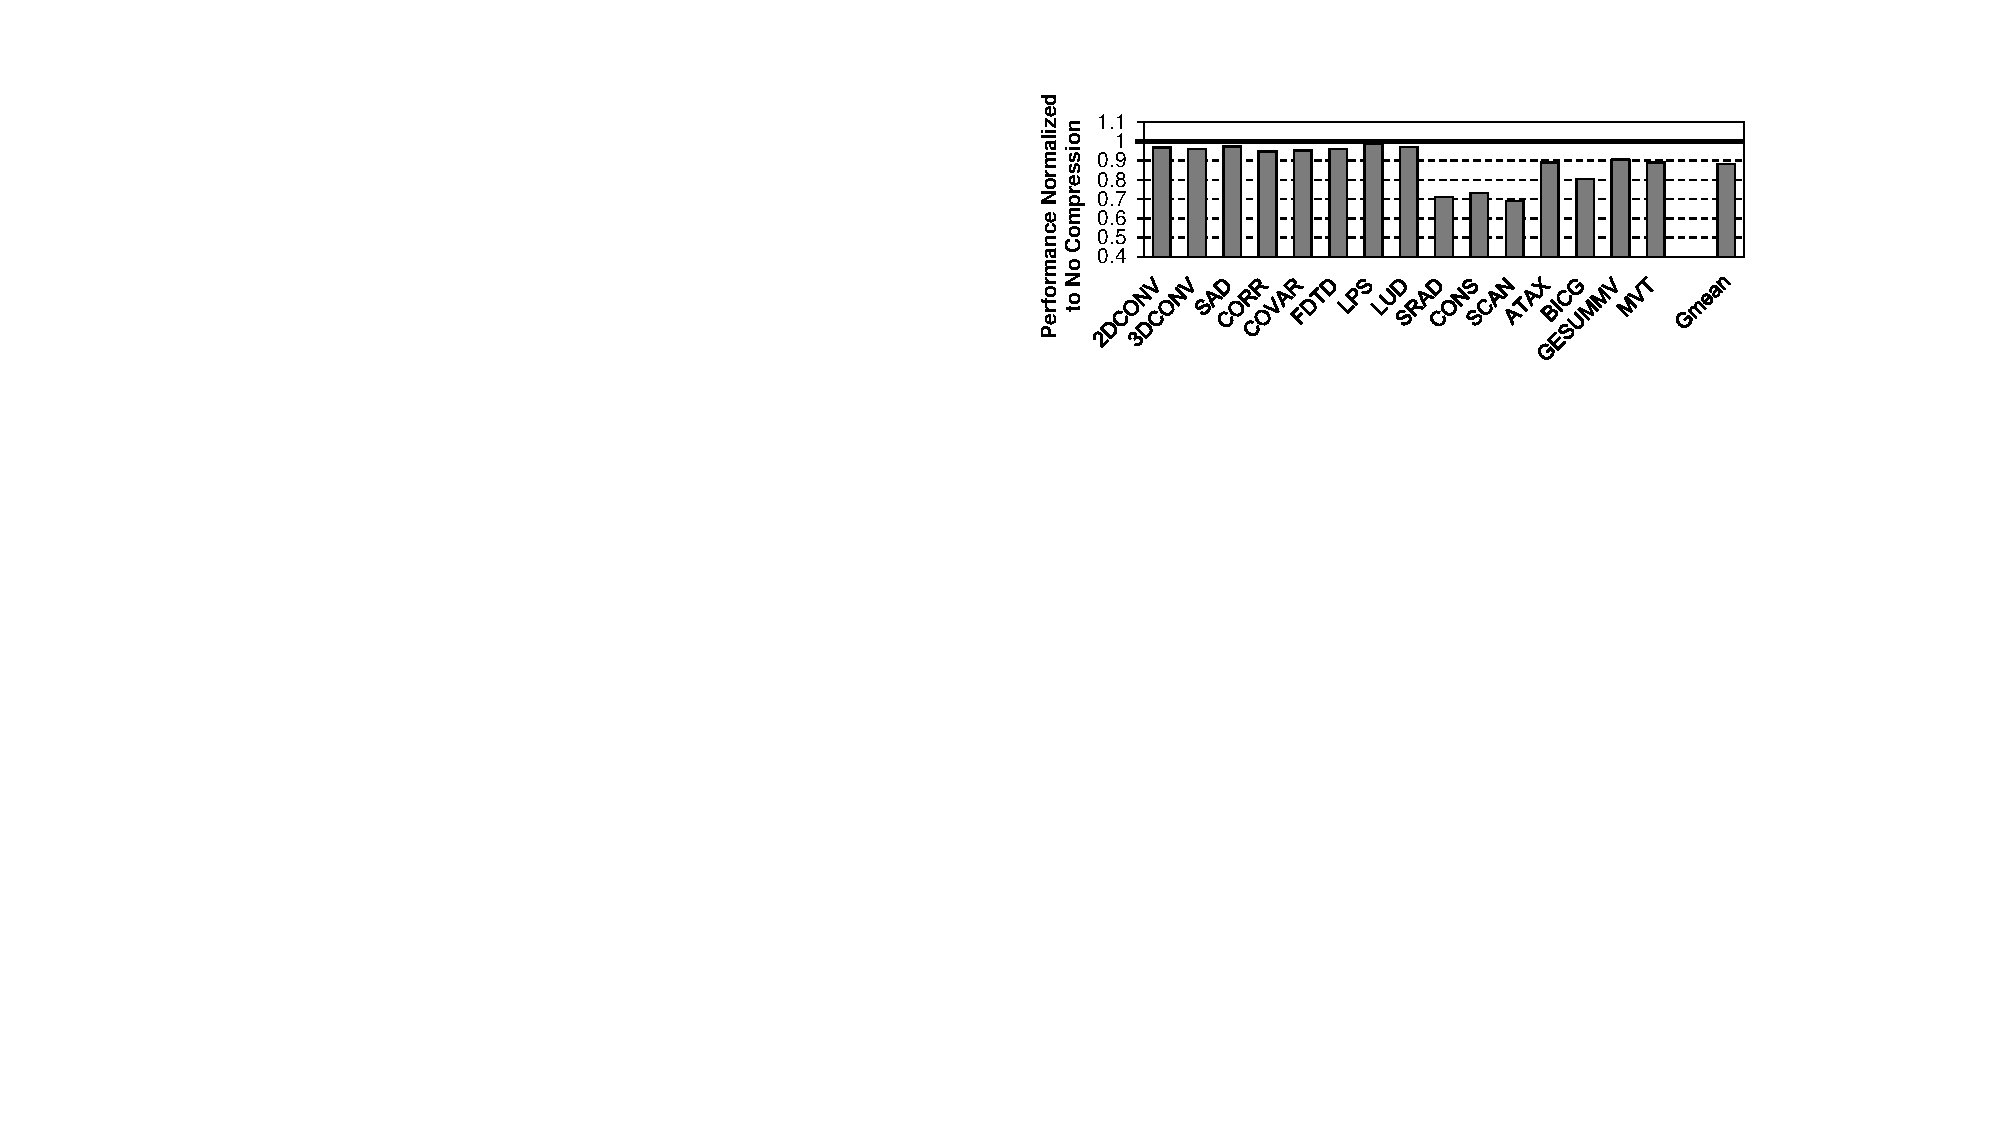
\includegraphics[width=\textwidth]{/Figs_ETC/data_compression_overhead}
  \caption{无限内存情况下的LCP内存容量压缩技术造成的性能损失}
  \label{fig:data_compression_overhead}
\end{figure}

因此,对于ETC来说确定何时采用LCP压缩技术非常重要。
内存容量压缩技术主要应用在两种类型的应用程序中,包括数据共享的规则应用程序和非规则应用程序。
因为来自这两种类别的应用程序的线程块会访问大量的数据,而内存压缩技术允许更多的数据存储在主存中。
更重要的是,有了内存容量压缩技术,内存感知的并行度控制方法能够一定程度上缓解并行度的下降,这样相比单独并行度控制,更多的线程可以同时执行。

\textbf{实现方案}。
由于当前的GPU已经在内存控制器和PCIe上应用了带宽压缩技术~\upcite{rhu2018compressing,kim2016bit,kwon2018case,sathish2012lossless,tegrax1}。
内存控制器和DMA单元已经配置了压缩和解压缩硬件模块~\upcite{tegrax1}。
为实现LCP压缩框架,ETC采用了一个具有512个存储单元的缓存在内存控制器中以加速压缩元数据的查询,能够一定程度上降低LCP的性能开销。
一旦应用程序划分单元确定当前执行的应用程序是数据共享的规则应用程序或者是非规则应用程序,同时内存处于超额配置状态,ETC开始进行内存容量压缩操作。
所有写入到GPU内存的数据将采用BDI压缩算法~\upcite{pekhimenko2012base}进行压缩,并通过LCP框架存入内存,非常简单高效~\upcite{pekhimenko2012base,caba,lcp-micro13,pekhimenko2016case,toggle-gena-cal}。

\subsection{ETC设计总结}
图~\ref{fig:Overview}是ETC的顶层设计方案,主要包括\texttt{应用划分单元},\texttt{主动数据页逐出单元}、\texttt{内存感知的并行度控制单元}、以及\texttt{主存容量压缩单元}。
当待分配的总数据量大于GPU的物理内存时,ETC将被激活,应用程序划分器将开始根据GPU的硬件信息和编译信息识别应用程序类型。
一旦应用程序被识别为规则应用程序,ETC将在GPU驱动的虚存管理单元开启主动数据页逐出功能。
如果应用程序有数据共享,则同时开启内存容量压缩技术。
如果应用程序被识别为非规则应用程序,ETC将同时开启内存感知的并行度控制技术和内存容量压缩技术,避免内存抖动现象的同时提升有效内存容量。

\begin{figure}[htbp] % use float package if you want it here
  \centering
  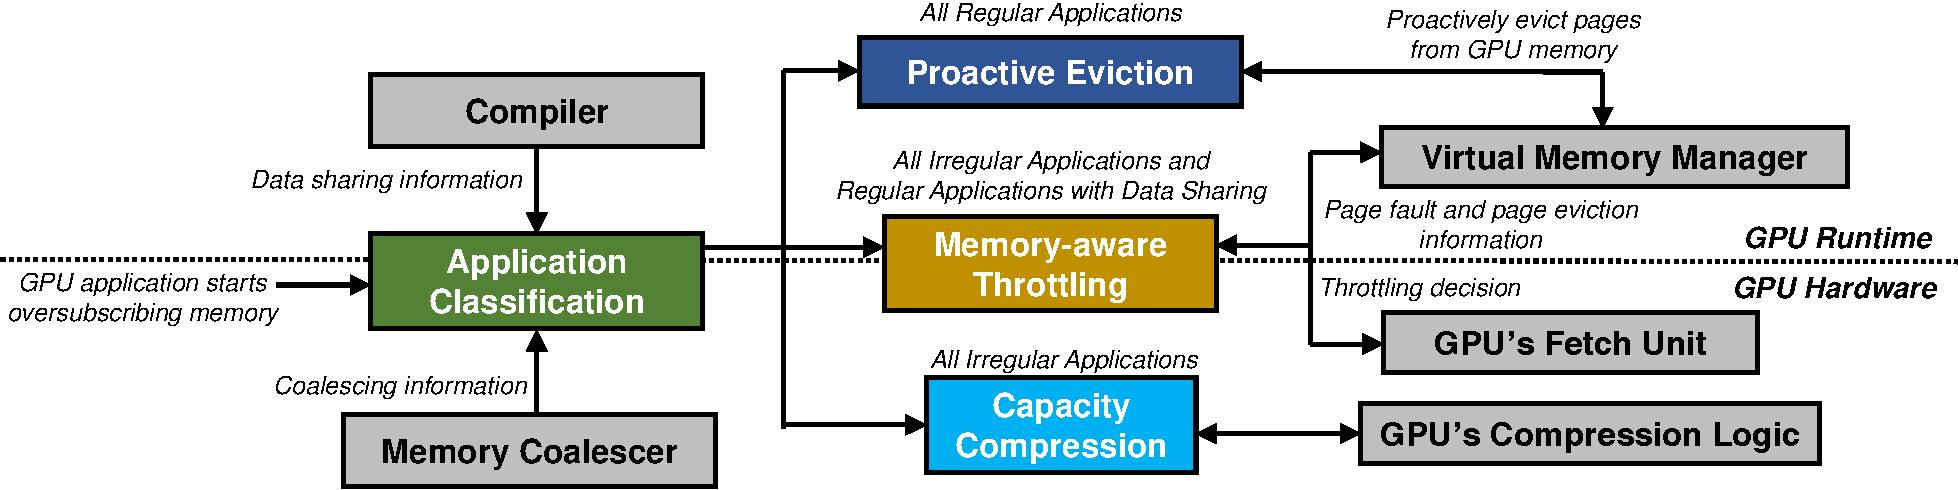
\includegraphics[width=\textwidth]{/Figs_ETC/Overview}
  \caption{ETC顶层设计图。包含四个模块,分别是应用程序类别划分单元、主动数据页逐出单元、内存感知的并行度控制单元和内存容量压缩单元。}
  \label{fig:Overview}
\end{figure}


\section{实验}
\label{sec:etcexperiment}

\subsection{实验方法}

我们修改了基于GPGPU-sim 3.2.2~\upcite{mafia,gpgpu-sim}的Mosaic模拟器~\upcite{mosaic.github,ausavarungnirun2017mosaic,Ausavarungnirun:2018:MRG:3173162.3173169}来评估ETC框架。
GPU核心和存储系统的实验配置如表~\ref{table:config}所示。

\begin{table}[h!]
\centering
\begin{tabular}{ll}
\hline \hline
\multicolumn{2}{c}{\textbf{GPU核心配置}} \\ \hline
\textbf{系统总览}           &  30个核心,每个核64个执行单元,8个存储分区\\
\textbf{核配置}           &  1020 MHz,9级流水线 \\ & 每个warp含64个线程,GTO warp调度~\upcite{rogers2012cache}\\
\textbf{私有一级缓存}    &  16KB,4路组相联,LRU \\ & L1缓存失效将合并请求发送到L2缓存\\
\textbf{私有一级TLB}    &  每个核心含64个条目,全相联,LRU\\
\textbf{共享二级缓存}   &  2MB,16路组相联,LRU \\ & 2个缓存块,每个内存块包含2个互连端口\\
\textbf{共享二级TLB}   &  总计512个条目,1路组相联,LRU,2端口\\
\textbf{页表查询缓存}    &  16路 8KB\\
\hline
\multicolumn{2}{c}{\textbf{存储配置}} \\
\hline
\textbf{DRAM内存}   & GDDR5 1674 MHz,8通道,每个Rank含8个Bank \\ & FR-FCFS调度~\upcite{fr-fcfs,frfcfs-patent},burst长度8\\
\textbf{页表查询}   & 64个线程共享页表查询器,查询四级页表\\
\textbf{统一虚拟内存配置} & 64KB数据页大小,2MB逐出数据大小\\ & 20$\mu$s 缺页中断处理时间, 16GB/s PCIe带宽  \\
                              
\hline
\end{tabular}
\caption{系统模拟配置}
\label{table:config}
\end{table}




\textbf{实时按需取页和内存超额配置}。
本章详尽地模拟了在CPU内存和GPU内存中实时按需取页数据迁移的过程,符合CUDA 8.0的描述。
当一个内核函数第一次要访问一块数据页时,TLB缺失会触发页表查询。
如果该数据页并不在GPU内存中时,页表查询失败,产生一个缺失页。
内存管理单元会中断CPU来处理这个缺页错误。
我们采用20$\mu$s的延迟模拟缺页中断处理延迟,并应用了最新的硬件数据页预取器来降低缺页中断开销。
当GPU内存完全被用满之后,GPU驱动会通过基于时序的LRU页替换策略逐出旧的数据页以足够的空间拷贝新的数据页。
我们在实验中为每个应用程序配置完全足够的内存空间、应用程序所需内存的75\%和50\%。

\textbf{测试应用程序}。
本章随机广泛地从CUDA SDK~\upcite{cuda-sdk}、Rodinia~\upcite{rodinia}、Parboil~\upcite{parboil}和Polybench~\upcite{polybench}选择了15个应用程序。
我们将应用程序划分为无数据共享的规则应用程序(2DCONV、3DCONV、SAD、CORR、COVAR、FDTD和LPS)、
数据共享的规则应用程序(LUD、SRAD、CONS和SCAN)以及非规则应用程序(ATAX、BICG、GESUMMV和MVT)。
它们在运行过程中由应用程序划分单元在线划分类型。
这些应用所需的内存占用从7.28MB到22.5MB不等,平均值为22.5MB。
本章没有模拟更大的内存占用是因为模拟过大的内存占用会导致不可接受的模拟延迟。

\textbf{设计参数}。
ETC框架采用了不同的设计参数。
本章设置内存合并参数阈值为10个缓存行来划分规则应用程序和非规则应用程序。
本章设置2MB作为剩余GPU内存空间的阈值来触发主动数据页逐出技术。
本章设置并行度下降和并行度上升的程度为一次一个GPU核心,本章实验发现这个值能实现最高的性能。


\subsection{实验结果}
我们评估ETC,并将其与1)当代采用数据页预取的基准模型(BL)~\upcite{tianhao-hpca16}以及2)一个理想情况下有无限内存的模型作比较。

\subsubsection{性能结果}

图~\ref{fig:data_etc}显示了不同类别应用程序以无限内存的基准模型为性能标准的相对性能结果。
基于这些结果,我们得出了三点结论。
首先,ETC在降低内存超额配置开销上作用显著。
对于无数据共享的规则应用程序,其性能接近无限内存的基准模型情况。
这是因为通过我们的主动数据页逐出技术,这一类应用程序最主要开销来源的数据页逐出延迟可以被完全掩藏。
第二,我们发现数据共享的规则应用程序由于不同内核函数之间的同步,数据页的额外迁移不能完全避免,
但是ETC相比于当前采用数据页预取的基准模型依然平均提升了60.4\%的性能。
第三,对于非规则的应用程序,ETC相比采用数据页预取的基准模型依然提升了2.7倍。
我们给出结论,ETC框架对于内存超额配置的性能恢复非常有效。

\begin{figure}[htbp] % use float package if you want it here
  \centering
  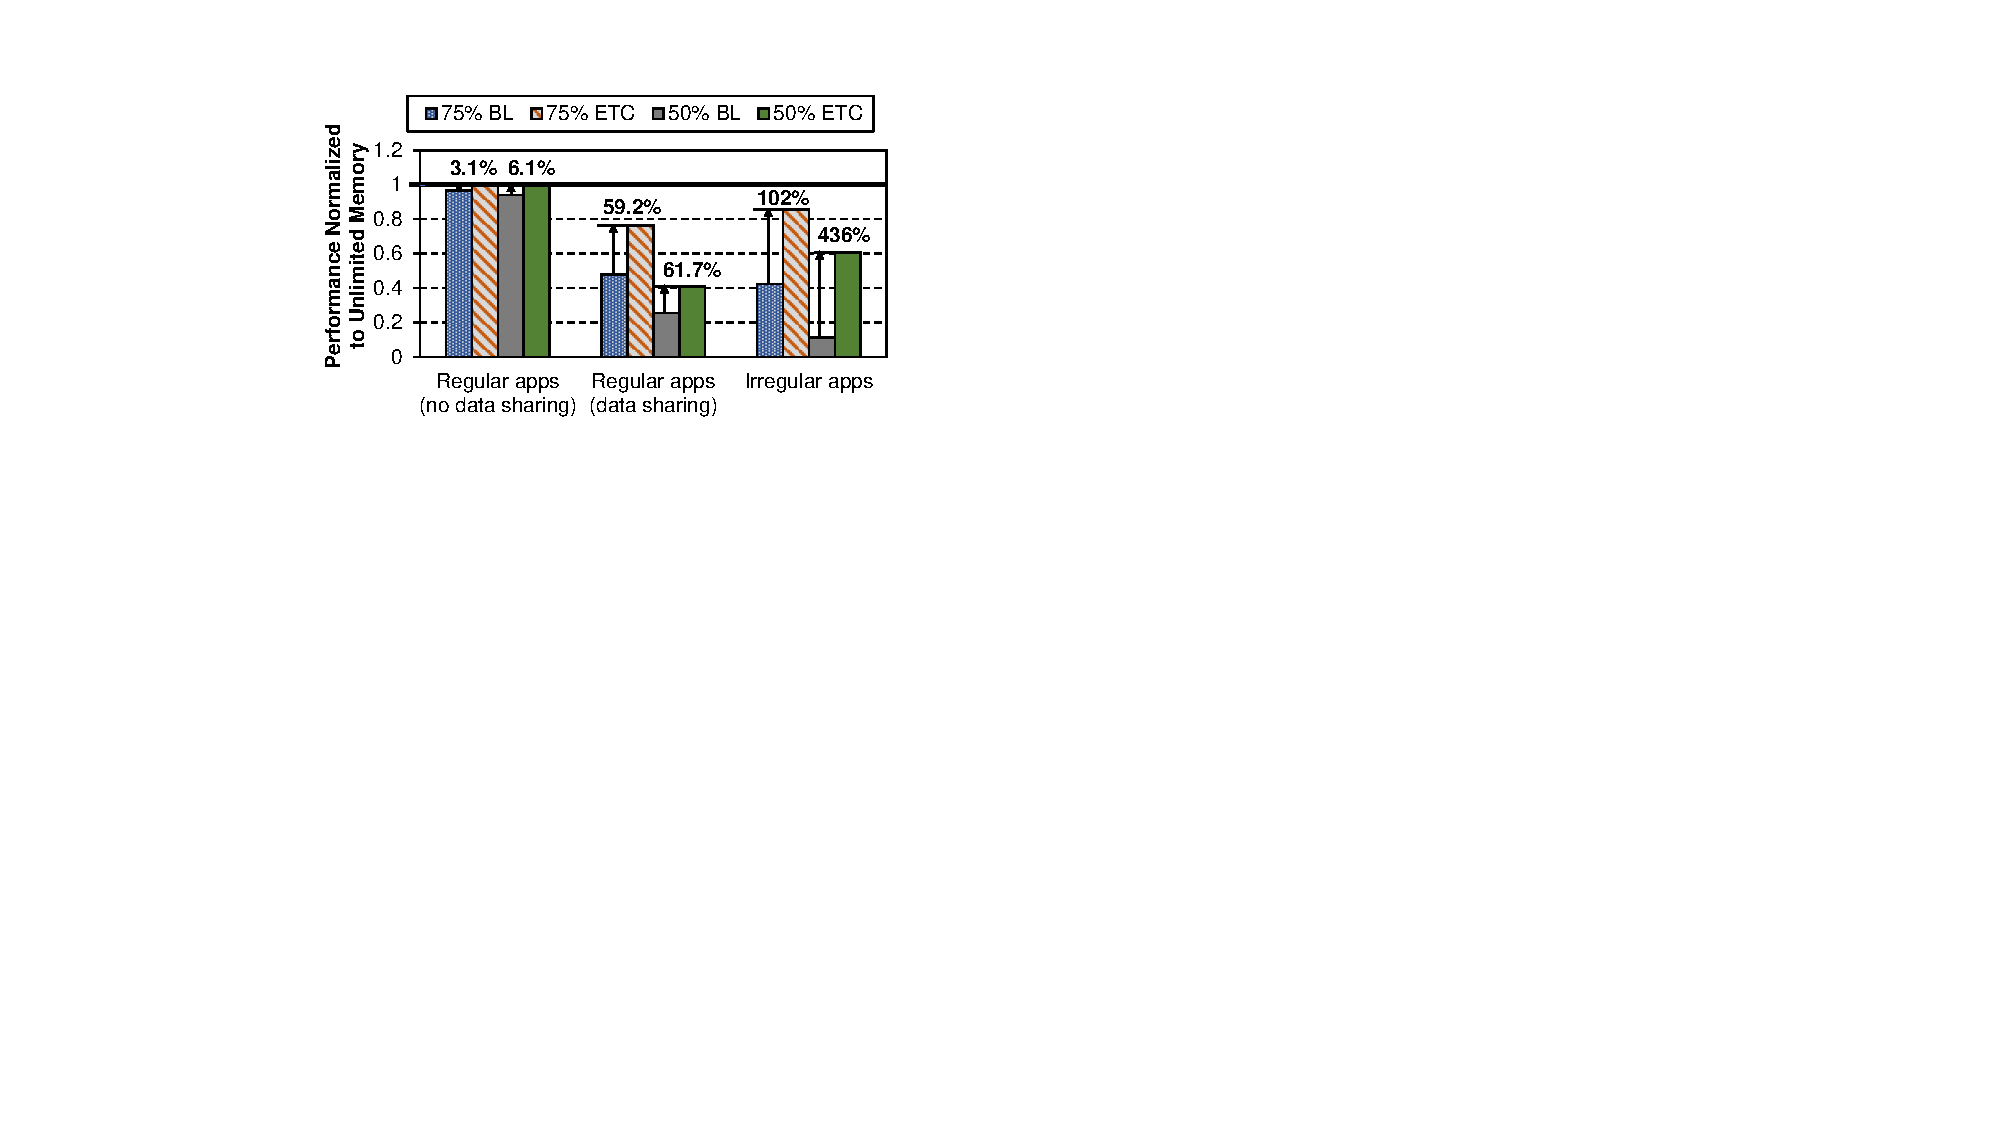
\includegraphics[width=0.8\textwidth]{/Figs_ETC/data_etc}
  \caption{ETC相对于无限内存的基准模型的性能}
  \label{fig:data_etc}
\end{figure}

\subsubsection{技术和应用程序细节分析}

本小节提供了关于ETC采用的不同技术对于每种类型应用程序影响的深度分析。

\textbf{无数据共享的规则应用程序}。
图~\ref{fig:data_non_shared_regular_app}显示了主动数据页逐出技术和容量压缩技术对于无数据共享的规则应用程序的影响。
我们得出三点观察。
第一,当主动数据页逐出技术被触发,数据页逐出延迟几乎可以完全被掩藏。
从实验中我们可以发现,对于无数据共享的规则应用程序中仅LPS因为逐出过多的数据页而导致性能离理想情况稍有下降。
第二,无数据共享的规则应用程序并不能从内存感知的并行度控制技术中获得性能提升,由于版面限制图~\ref{fig:data_non_shared_regular_app}并没有完全展现。
因为该类型的应用程序在线工作数据集本身就非常小,无需降低并行度。同时该类型应用程序的主要开销来源为等待数据页逐出的延迟。
事实上,内存感知的并行度控制技术使得线程级并行下降的同时,延迟掩藏能力也会差距。
第三,无数据共享的规则应用程序在采用了内存压缩技术后,性能比基准模型更低。
这是因为额外的压缩相关元数据访问所带来的开销,这在~\ref{compress}节已详细介绍的。


\begin{figure}[htbp] % use float package if you want it here
  \centering
  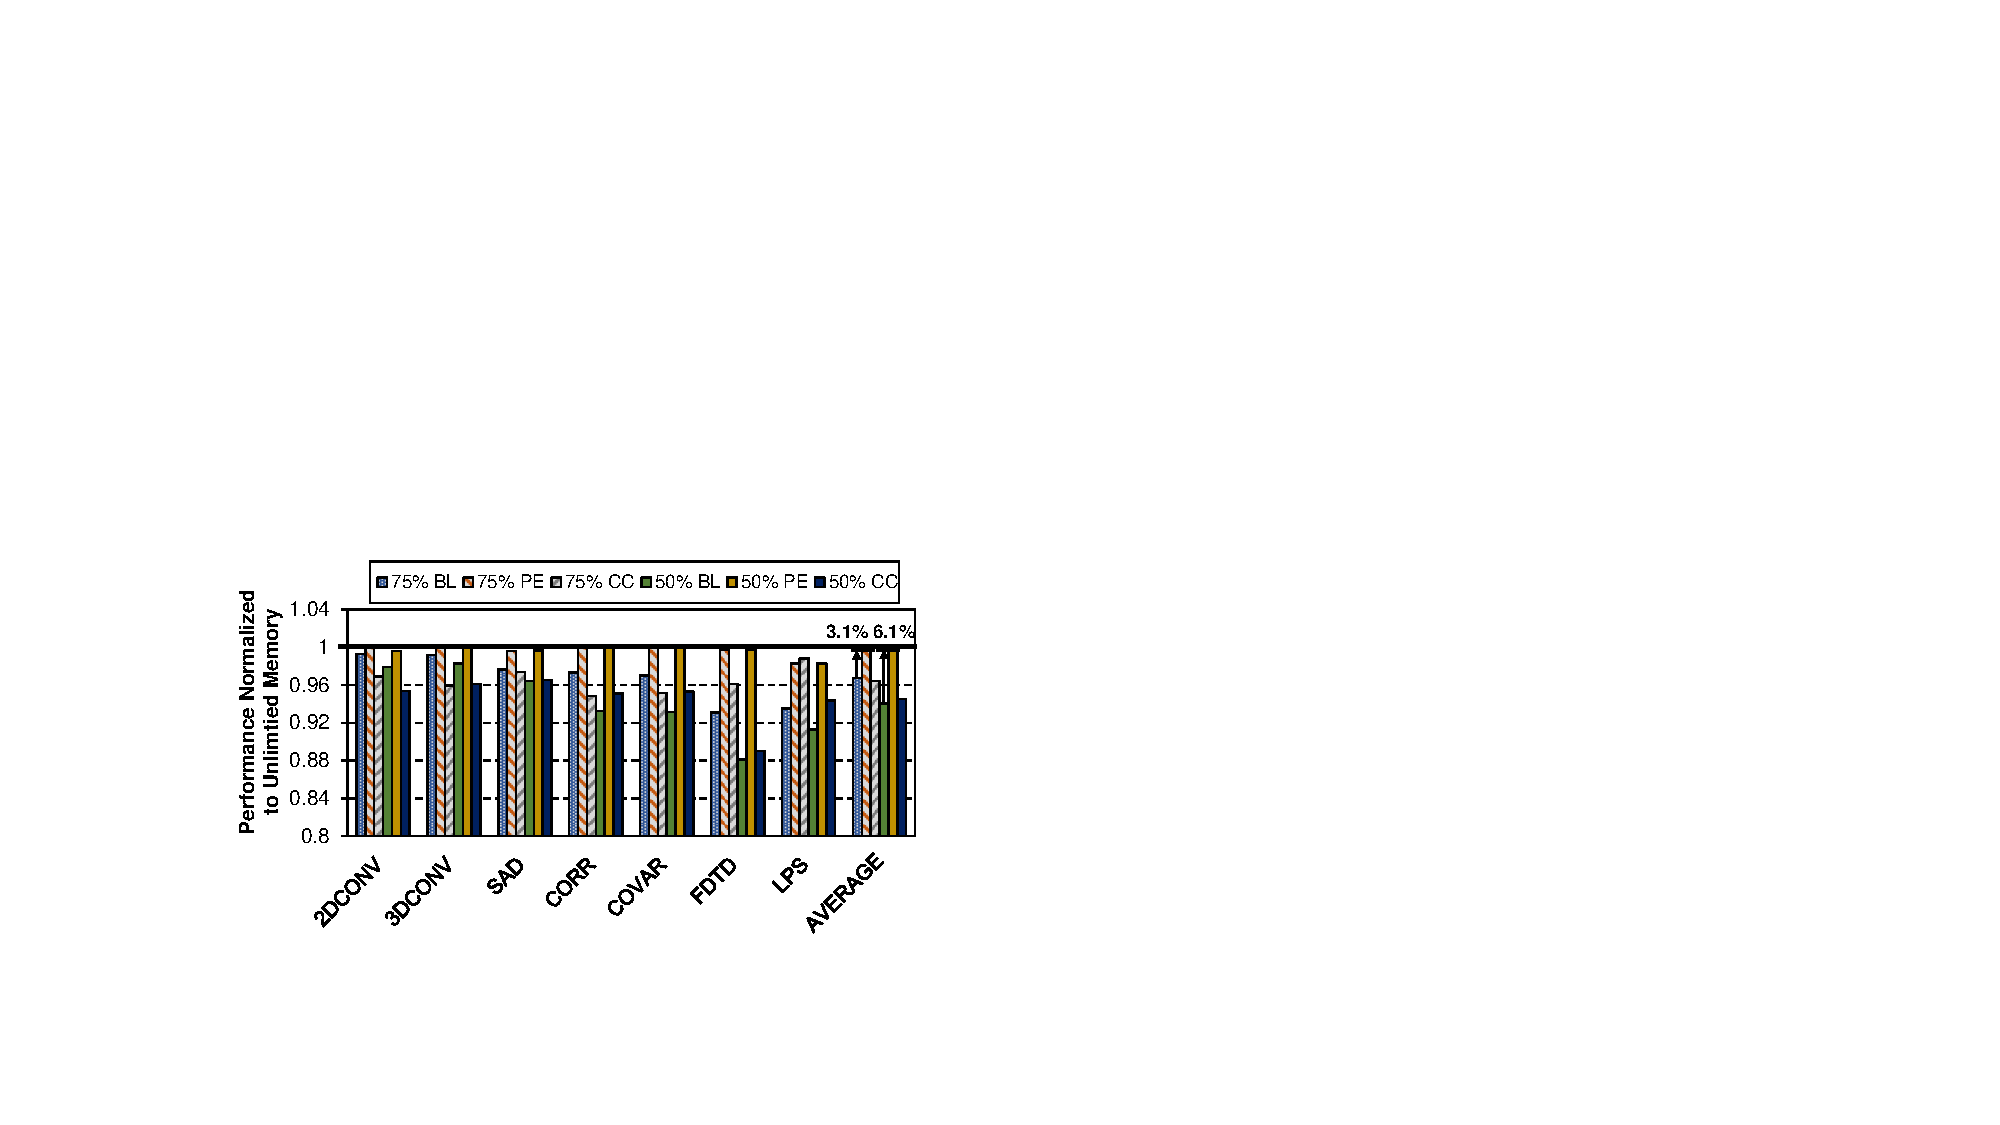
\includegraphics[width=0.8\textwidth]{/Figs_ETC/data_non_shared_regular_app}
  \caption{无数据共享的规则应用程序的性能}
  \label{fig:data_non_shared_regular_app}
\end{figure}

\textbf{数据共享的规则应用程序}。
图~\ref{fig:data_PE+CC}显示了数据共享的规则应用程序在主动数据页逐出技术、容量压缩技术和二者一起使用时的性能。
本章得出了四点观察。
第一,与无限内存的理想基准情况相比,数据页预取的基准模型在75\%和50\%的数据集能被物理内存容纳的情况下性能分别下降了52.2\%和74.1\%。
第二,仅采用主动数据页逐出技术,性能相比于基准模型仅提升了9.3\%。
这是因为由于数据共享导致的数据移动在这种情况下是内存超额配置的最主要开销。
第三,仅使用内存压缩技术可以获得52.8\%的性能提升。
这是因为它增加了有效内存容量。
第四,当主动数据页逐出技术和内存压缩技术同时使用时,平均可以获得60.4\%的性能提升。
本章得出以下结论,无论数据是否在多个内核函数之间共享,ETC框架都能够提升规则应用程序的性能。

\begin{figure}[htbp] % use float package if you want it here
  \centering
  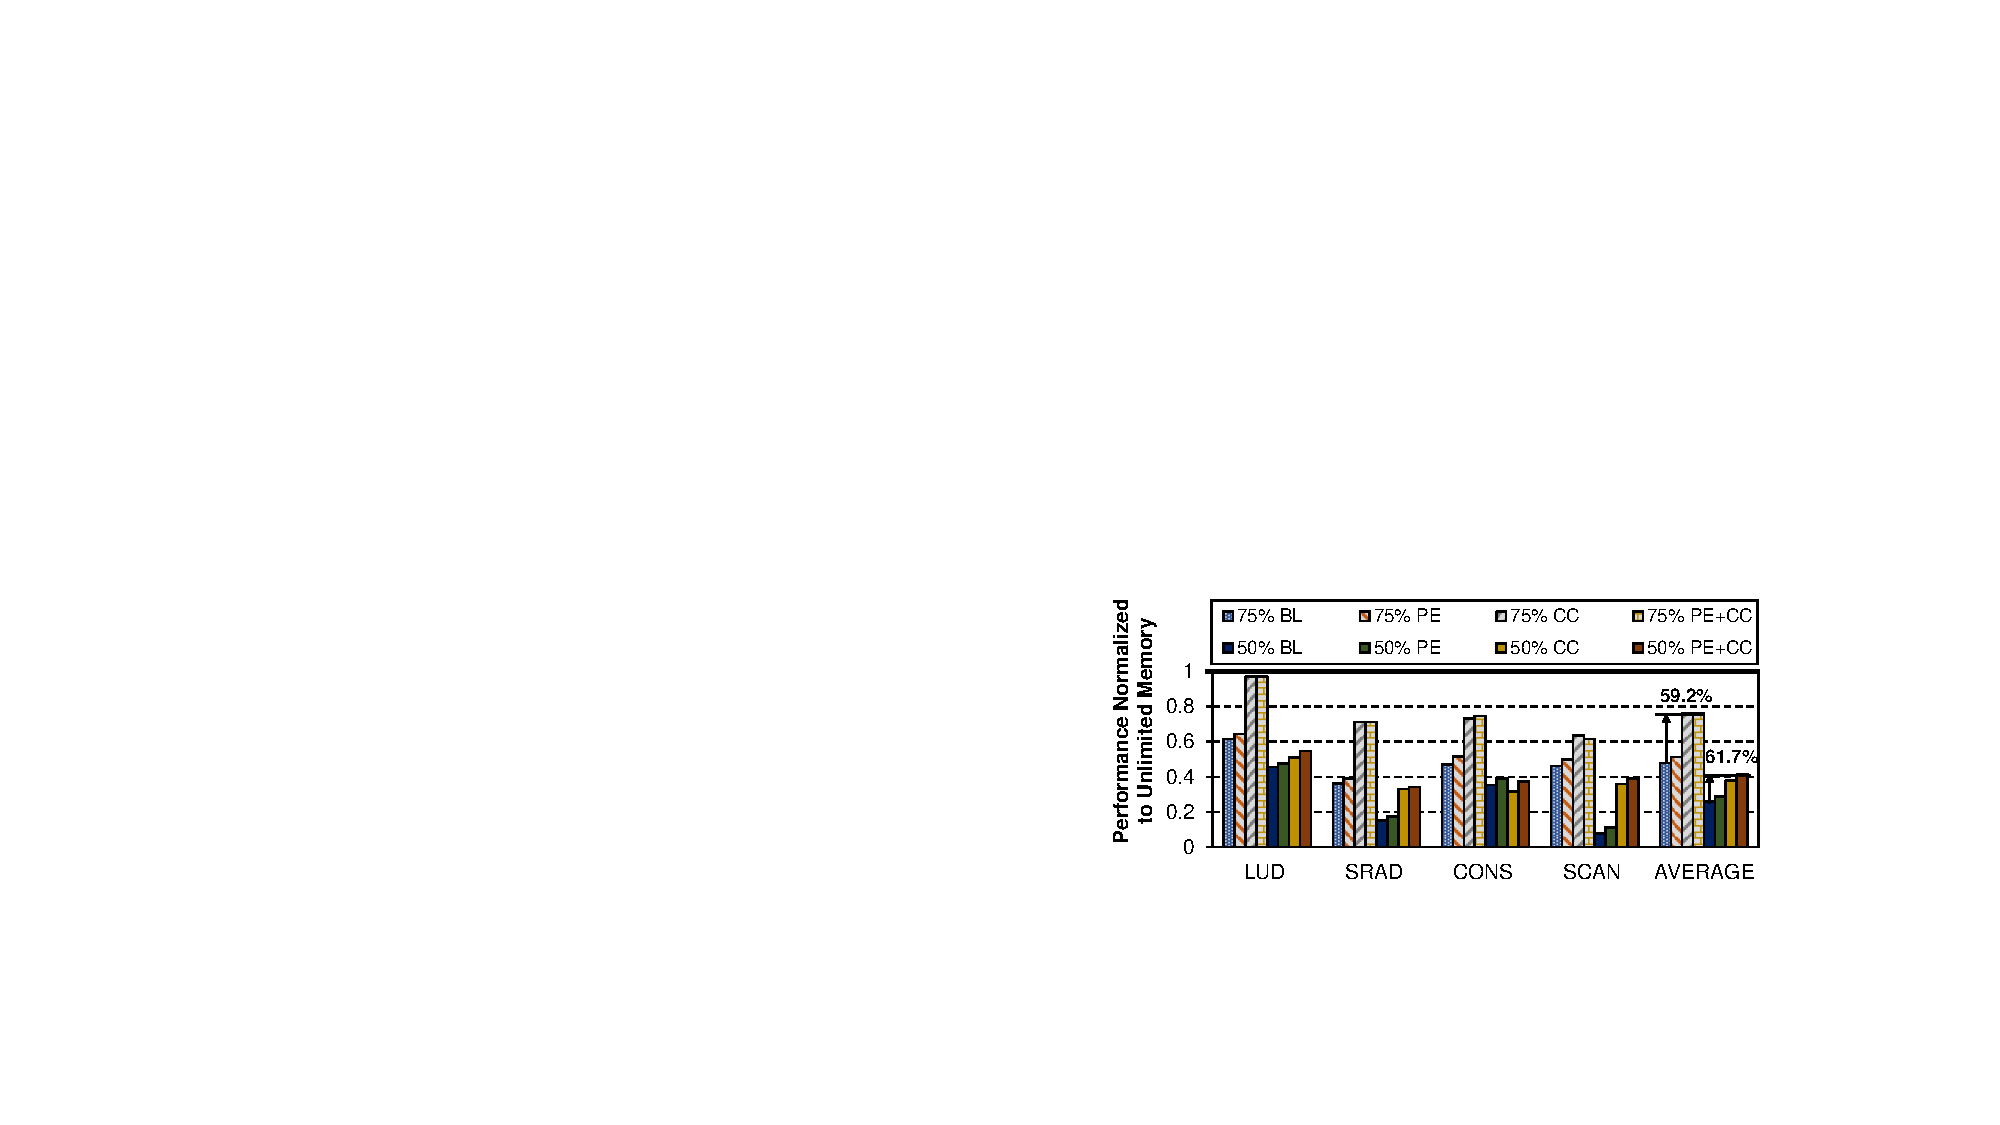
\includegraphics[width=0.8\textwidth]{/Figs_ETC/data_PE+CC}
  \caption{数据共享的规则应用程序的性能}
  \label{fig:data_PE+CC}
\end{figure}


\textbf{非规则应用程序}。
图~\ref{fig:data_num_eviction_75}和图~\ref{fig:data_num_eviction_50}显示了每个非规则应用程序在ETC各个技术下的性能和总的数据页逐出次数。
为评估ETC框架的并行度控制策略(MT),我们将它和一个简单的并行度控制策略进行比较,该策略静态地在开始执行时减少一半的GPU核心数量(如图~\ref{fig:data_num_eviction_75}和图~\ref{fig:data_num_eviction_50}所示)。
本章得出了三点观察。
首先,简单的并行度控制方法在内存能容纳75\%的数据集的情况下性能提升57.7\%。
第二,当内存仅能容纳50\%的数据集的时候,简单的并行度控制方法变得不那么有效,降低了10.5\%的性能。
相反地,我们的内存感知策略,可以动态地调整可运行的GPU核心数量。
相比于当前的基准模型,我们的内存感知策略提升了436\%的性能。
第三,在BICG和GESUMMV两个应用程序内存容量仅能容纳75\%的数据集的情况下,ETC的自适应调整的并行度控制策略性能不及简单的并行度控制方法。
这是因为自适应调整需要一段时间才能达到最佳并行级别,而简单的并行度控制方法在这种情况恰好一次性达到了较好的并行级别。



\begin{figure}[htbp] % use float package if you want it here
  \centering
  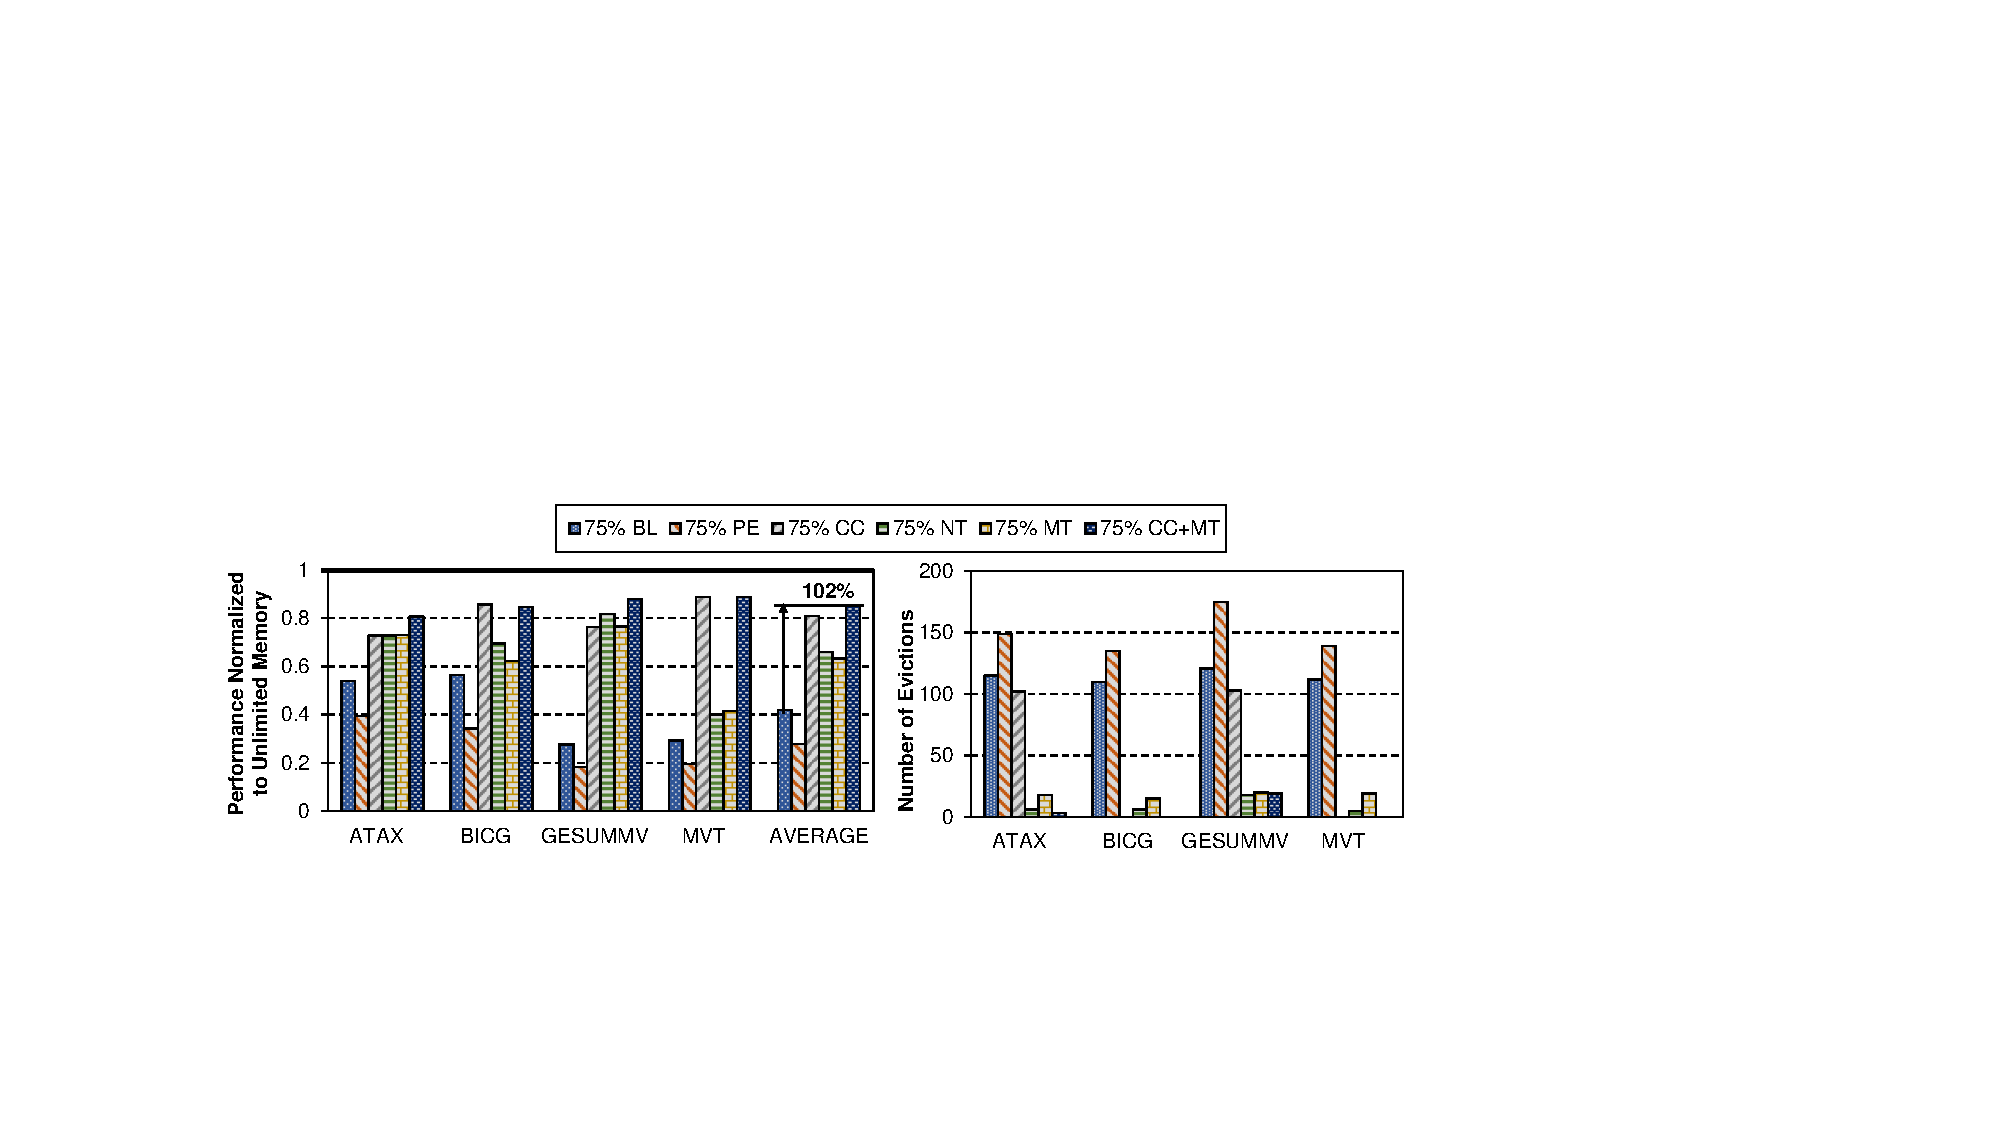
\includegraphics[width=\textwidth]{/Figs_ETC/data_num_eviction_75}
  \caption{非规则应用程序的性能(75\%的内存占用可以被容纳进内存)}
  \label{fig:data_num_eviction_75}
\end{figure}

\begin{figure}[htbp] % use float package if you want it here
  \centering
  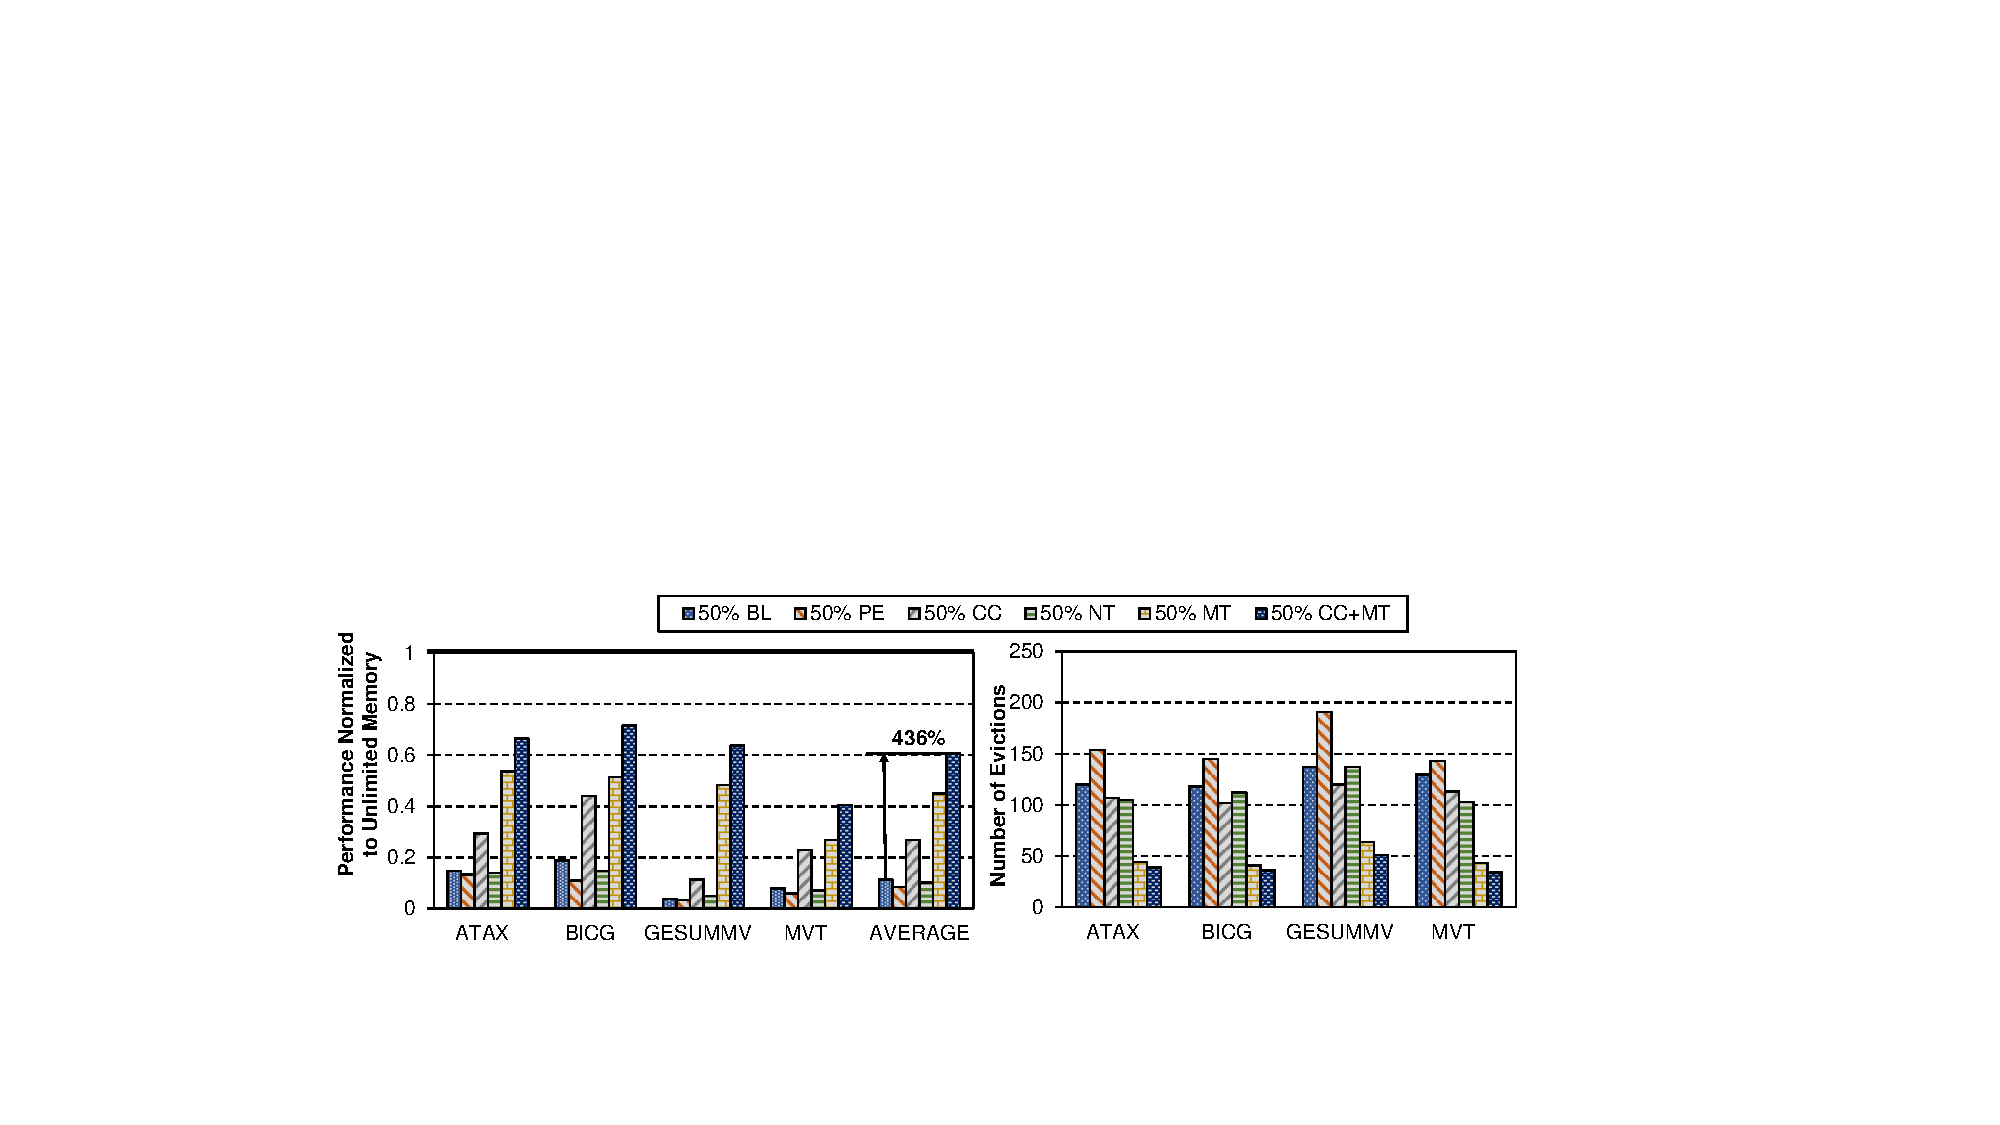
\includegraphics[width=\textwidth]{/Figs_ETC/data_num_eviction_50}
  \caption{非规则应用程序的性能(50\%的内存占用可以被容纳进内存)}
  \label{fig:data_num_eviction_50}
\end{figure}

图~\ref{fig:ATAX_page_fault_rate}显示了1000万个时钟周期里非规则应用程序ATAX的缺页中断率。
当内存超额配置且75\%的数据集能存放于内存中,会发生内存抖动现象,且频繁地发生缺页中断。
相反地,当内存感知的并行度控制方法被激活时,缺页中断并不频繁。
这说明我们的内存感知的并行度控制方法对于降低在线工作数据集的大小非常有效。
同时,图~\ref{fig:data_num_eviction_75}和图~\ref{fig:data_num_eviction_50}的数据页表明,内存感知的并行度控制方法可以减少数据页逐出的发生。


\begin{figure}[htbp] % use float package if you want it here
  \centering
  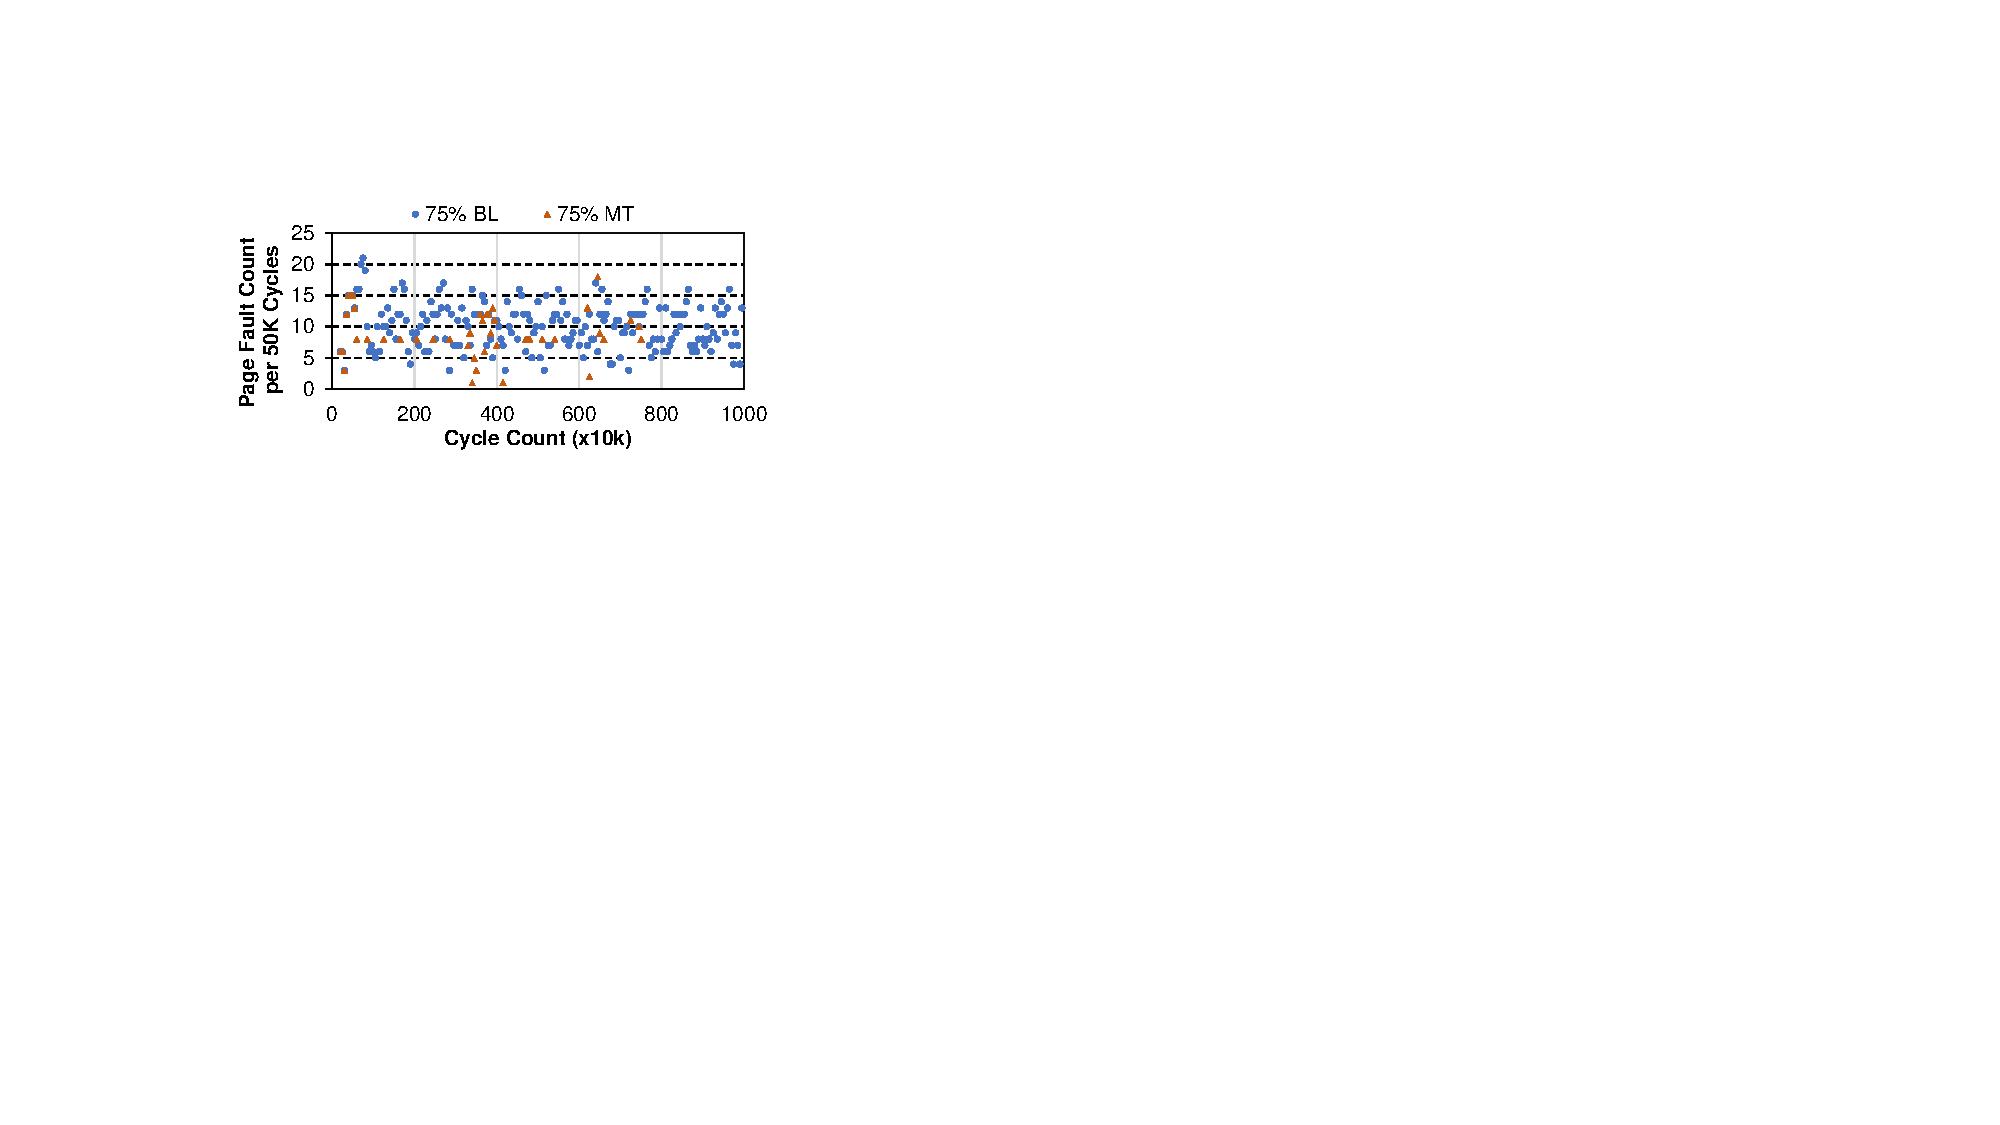
\includegraphics[width=0.8\textwidth]{/Figs_ETC/ATAX_page_fault_rate}
  \caption{ATAX的缺页中断率变化趋势}
  \label{fig:ATAX_page_fault_rate}
\end{figure}


内存容量压缩策略对于非规则应用程序的有效程度取决于压缩率和GPU相对于应用程序的内存占用的比例。
当一个应用程序完整的内存占用能够在压缩之后被物理内存容纳,缺页中断将不再发生。
图~\ref{fig:data_num_eviction_75}中BICG和MVT显著减少的数据页逐出数目说明这两个应用程序的压缩率足够高,使得内存能够完全容纳应用程序的内存占用。
相比于当前的数据页预取基准模型,内存压缩技术分别提升了51.8\%和203.6\%。
相比于无限内存的理想基准情况,BICG和MVT分别恢复了85.7\%和88.7\%的性能。
图~\ref{fig:data_num_eviction_50}显示了GPU的内存仅能容纳50\%的数据集的性能情况。
即使使用了内存容量压缩技术,所有的应用程序都出现了内存抖动。
我们的内存感知的并行度控制技术在和内存容量压缩技术同时使用时,相比于当前基准情况的性能提升了436\%。
我们得出以下结论,采用内存容量压缩技术有助于提升内存超额配置下非规则应用程序的性能,然而缺页中断和内存抖动仍然会限制应用程序的性能。
因此,需要内存容量压缩技术和内存感知的并行度控制一起工作以在内存超额配置的情况下达到较好的性能。

我们观察到主动数据页逐出技术相比于被动数据页逐出技术性能下降了29.7\%。
这是因为数据页被过早地逐出GPU物理内存。
因此,主动数据页逐出技术并不适合非规则应用程序。

总的来说,内存感知的并行度控制技术和内存容量压缩技术对于提升非规则应用程序的性能非常有效。
因此,我们的ETC框架采用这两种技术来提升非规则应用程序的性能。
如图~\ref{fig:data_num_eviction_75}和图~\ref{fig:data_num_eviction_50}所示,采用了这两种技术的ETC框架能够提升270\%的非规则应用程序的性能。
虽然并行度控制技术在一定程度上降低了线程级并行,但它能够有效降低内存超额配置的开销以及缓解内存抖动。

\subsection{应用程序划分的精确度分析}
ETC框架依赖于正确的应用程序类别划分。
只有确定正确的应用程序类别才能选择最合适的策略(见~\ref{AC})。
图~\ref{fig:data_coalesce_factor}比较了从5万个时钟周期取样的平均访存合并系数与每个应用程序的真实平均访存合并系数。
我们可以观察到规则应用程序和非规则应用程序的访存合并系数相差非常大。
我们发现,将访存合并系数阈值设置在5到10之间都能使得ETC的应用程序类别划分准确读达到100\%。
因此在本课题研究中我们将阈值设置为10。

\begin{figure}[htbp] % use float package if you want it here
  \centering
  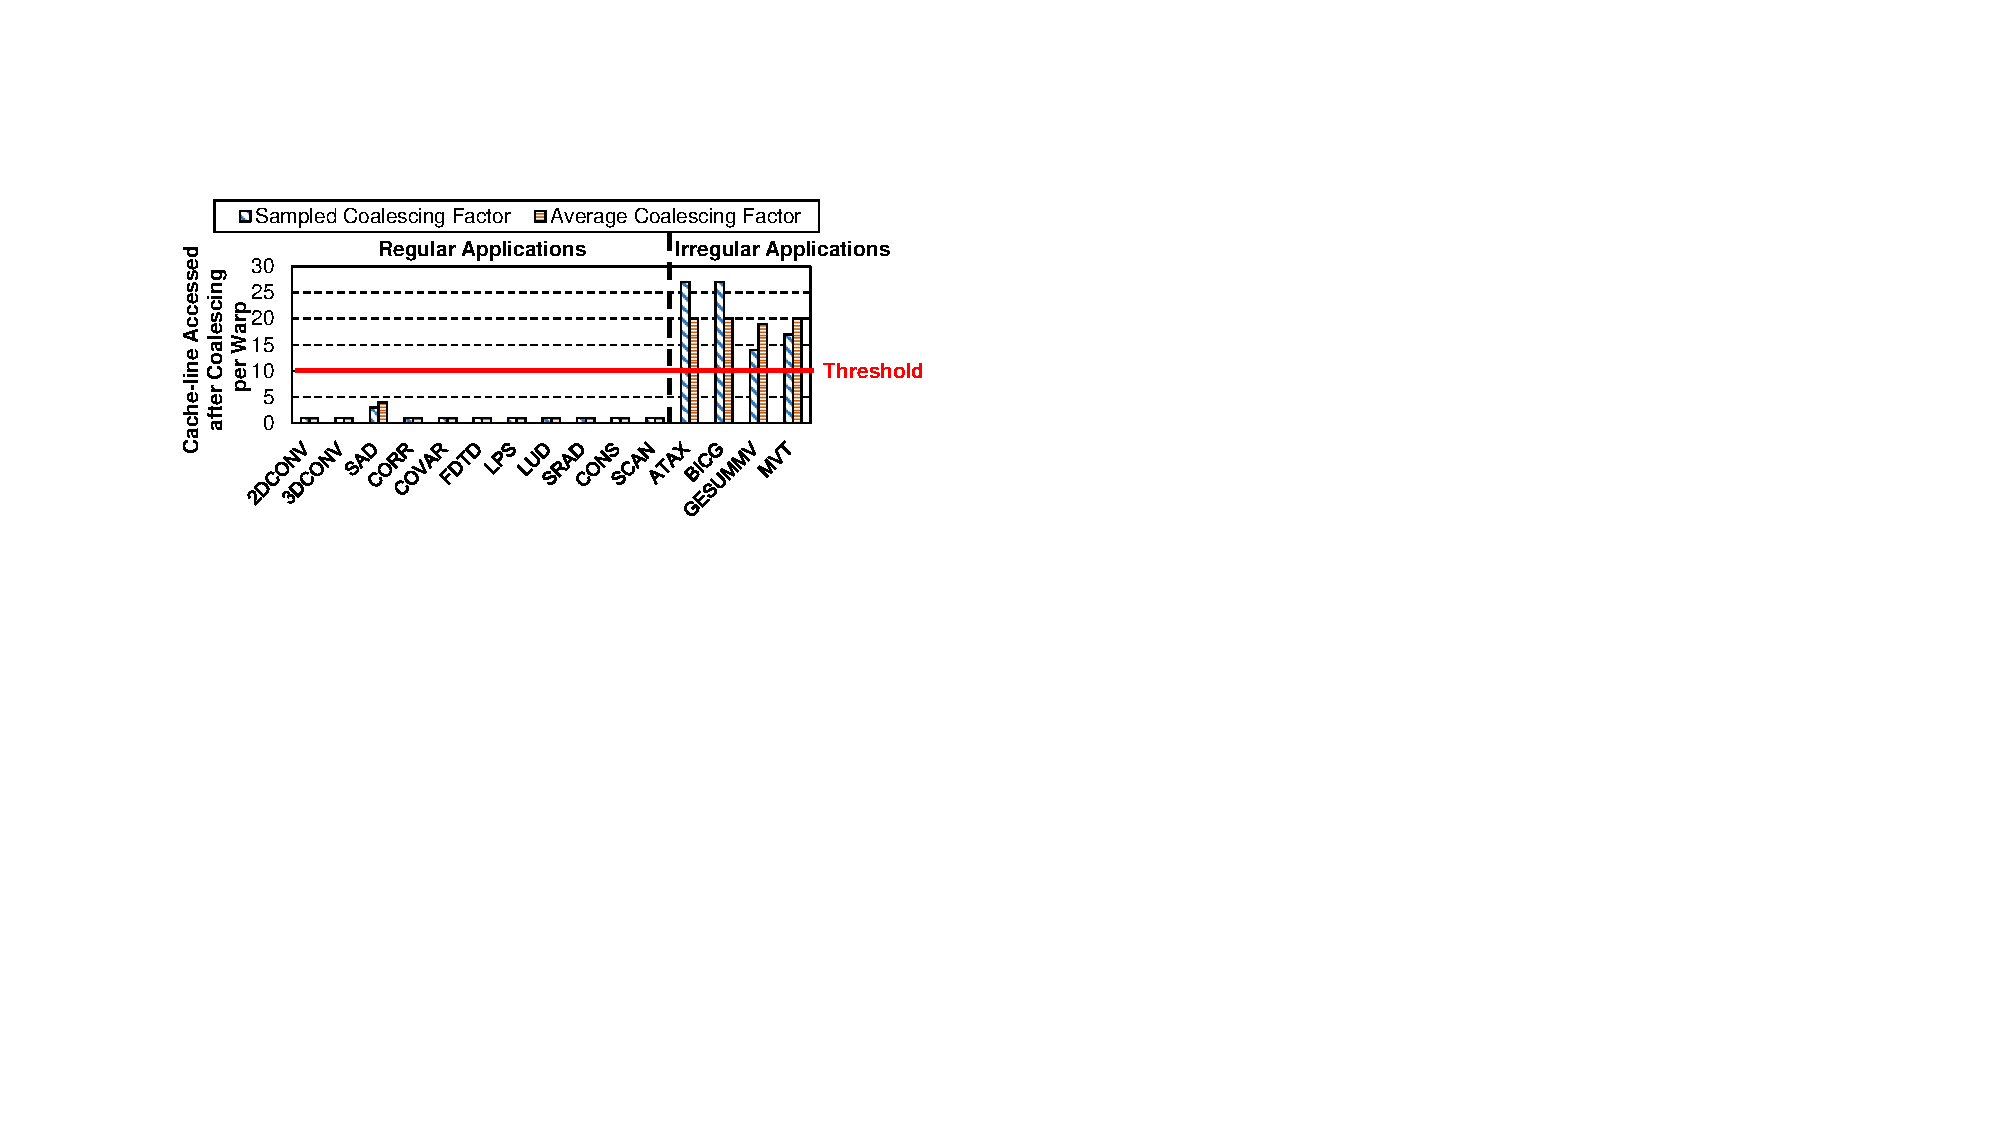
\includegraphics[width=0.8\textwidth]{/Figs_ETC/data_coalesce_factor}
  \caption{不同应用程序的访存合并系数(缓存行合并)}
  \label{fig:data_coalesce_factor}
\end{figure}


图~\ref{fig:data_page_coalesce_factor}显示了每个warp指令中32个线程访问的平均数据页数目。
我们发现非规则应用程序的warp一般会访问多个数据页,而几乎大多数的规则应用程序一般只访问一个数据页。
因此,采用数据页级别的访存合并系数与缓存行级别的访存合并系数来判定不同的应用程序类别均有非常高的准确率。

\begin{figure}[htbp] % use float package if you want it here
  \centering
  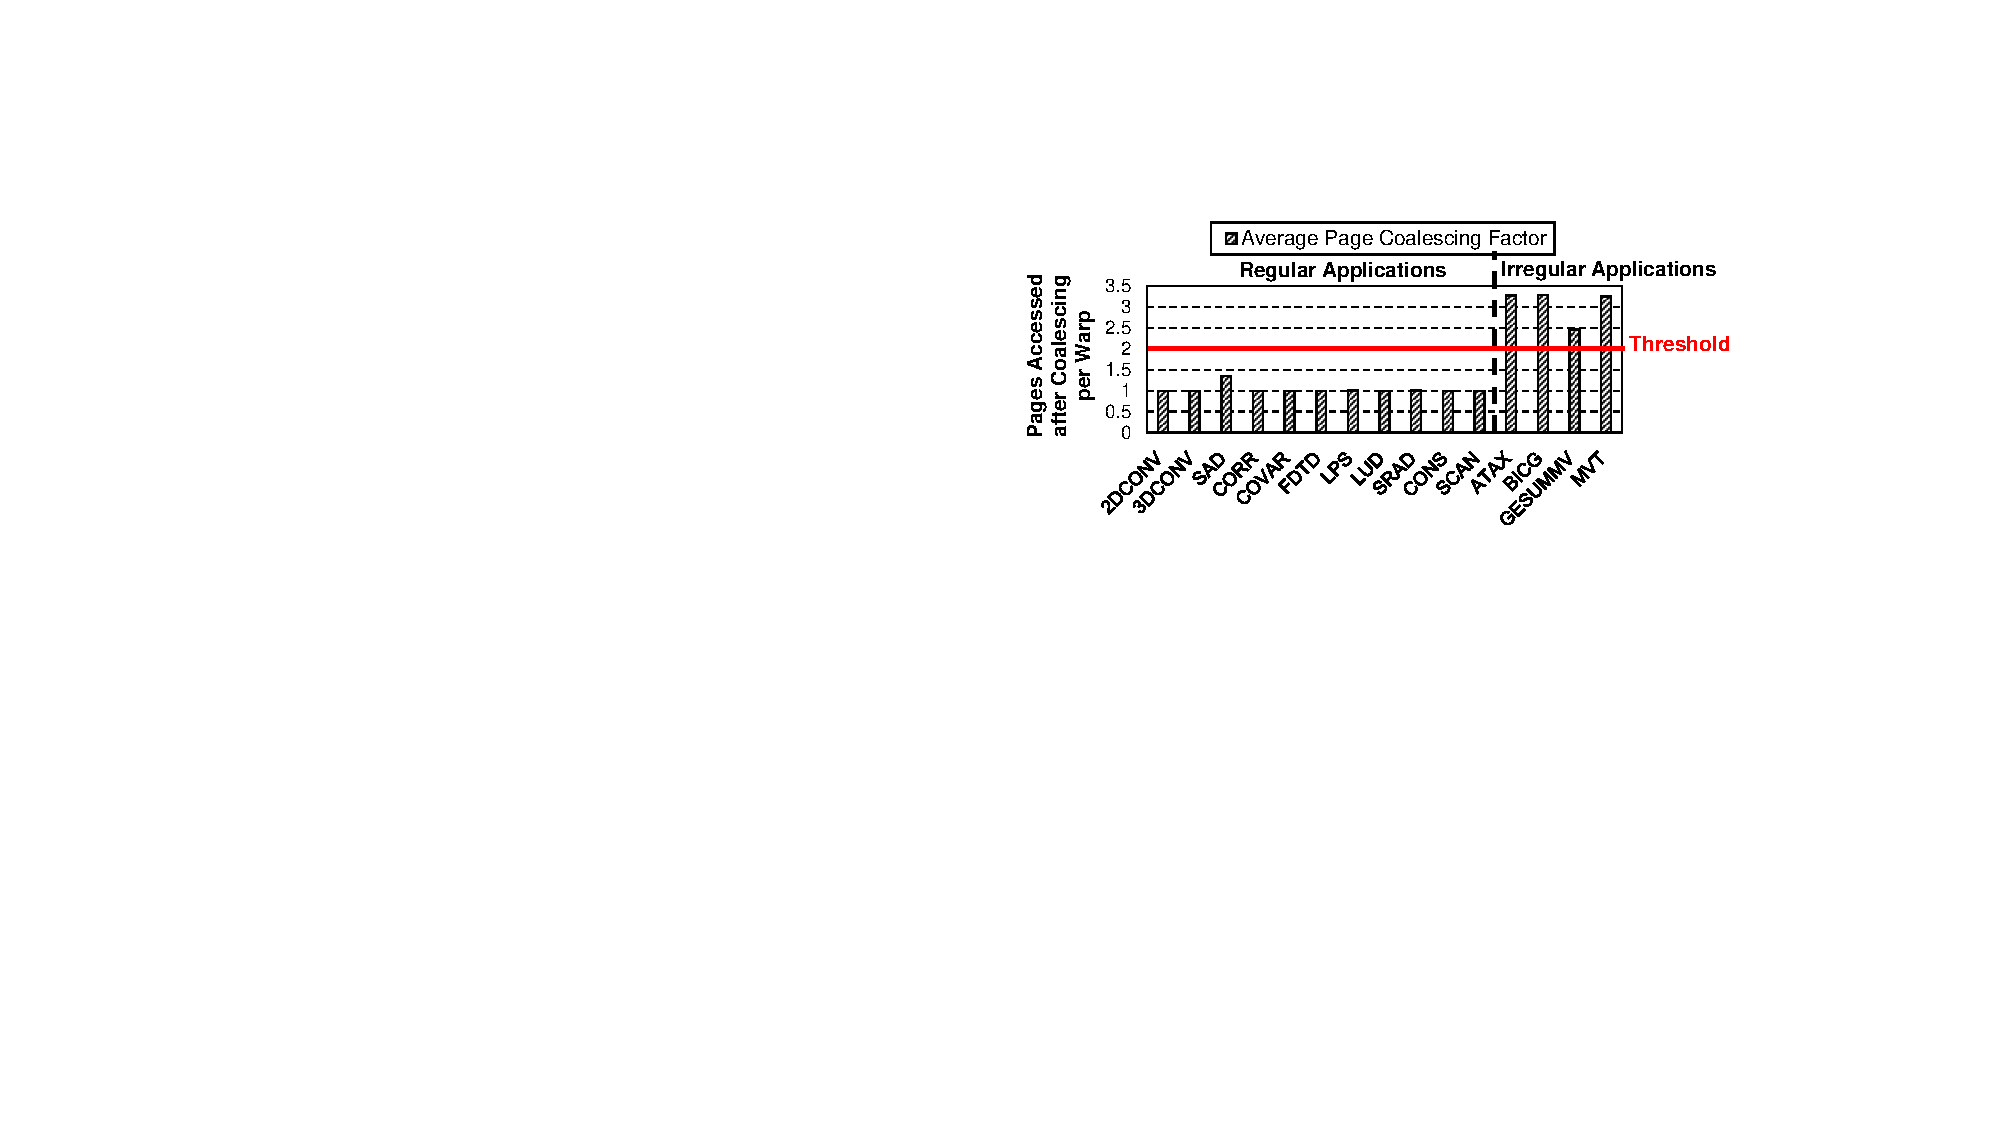
\includegraphics[width=0.8\textwidth]{/Figs_ETC/data_page_coalesce_factor}
  \caption{不同应用程序的访存合并系数(数据页合并)}
  \label{fig:data_page_coalesce_factor}
\end{figure}

\subsection{敏感度分析}
在这一节我们测试了不同敏感度下ETC框架的性能。
主要包括内存感知的并行度控制策略中调节粒度大小、缺页中断处理延迟大小和内存容量大小对GPU内存超额配置下的性能影响。

\textbf{内存感知的并行度控制度}。
每个阶段并行度提高或降低所变化的GPU核心的数量称为并行度控制的度。
它能够直接影响应用程序的性能。
图~\ref{fig:data_throttle_SMs_sensitive}和图~\ref{fig:data_release_SMs_sensitive}显示了每个阶段调节不同的GPU核心数(每次增加或减少的GPU核心数量)的相对性能。
基于图~\ref{fig:data_throttle_SMs_sensitive}和图~\ref{fig:data_release_SMs_sensitive},可以得出两点观察。
第一,ETC的内存感知的并行度控制策略在并行度下降和上升度均为1时得到最高的性能。
这说明细粒度的调整效果最好;
第二,相比于并行度上升,我们观察到ETC框架的性能对于并行度下降更加敏感,因为缺页中断产生的开销相比于线程级并行的下降产生的开销更大。

\begin{figure}[htbp] % use float package if you want it here
  \centering
  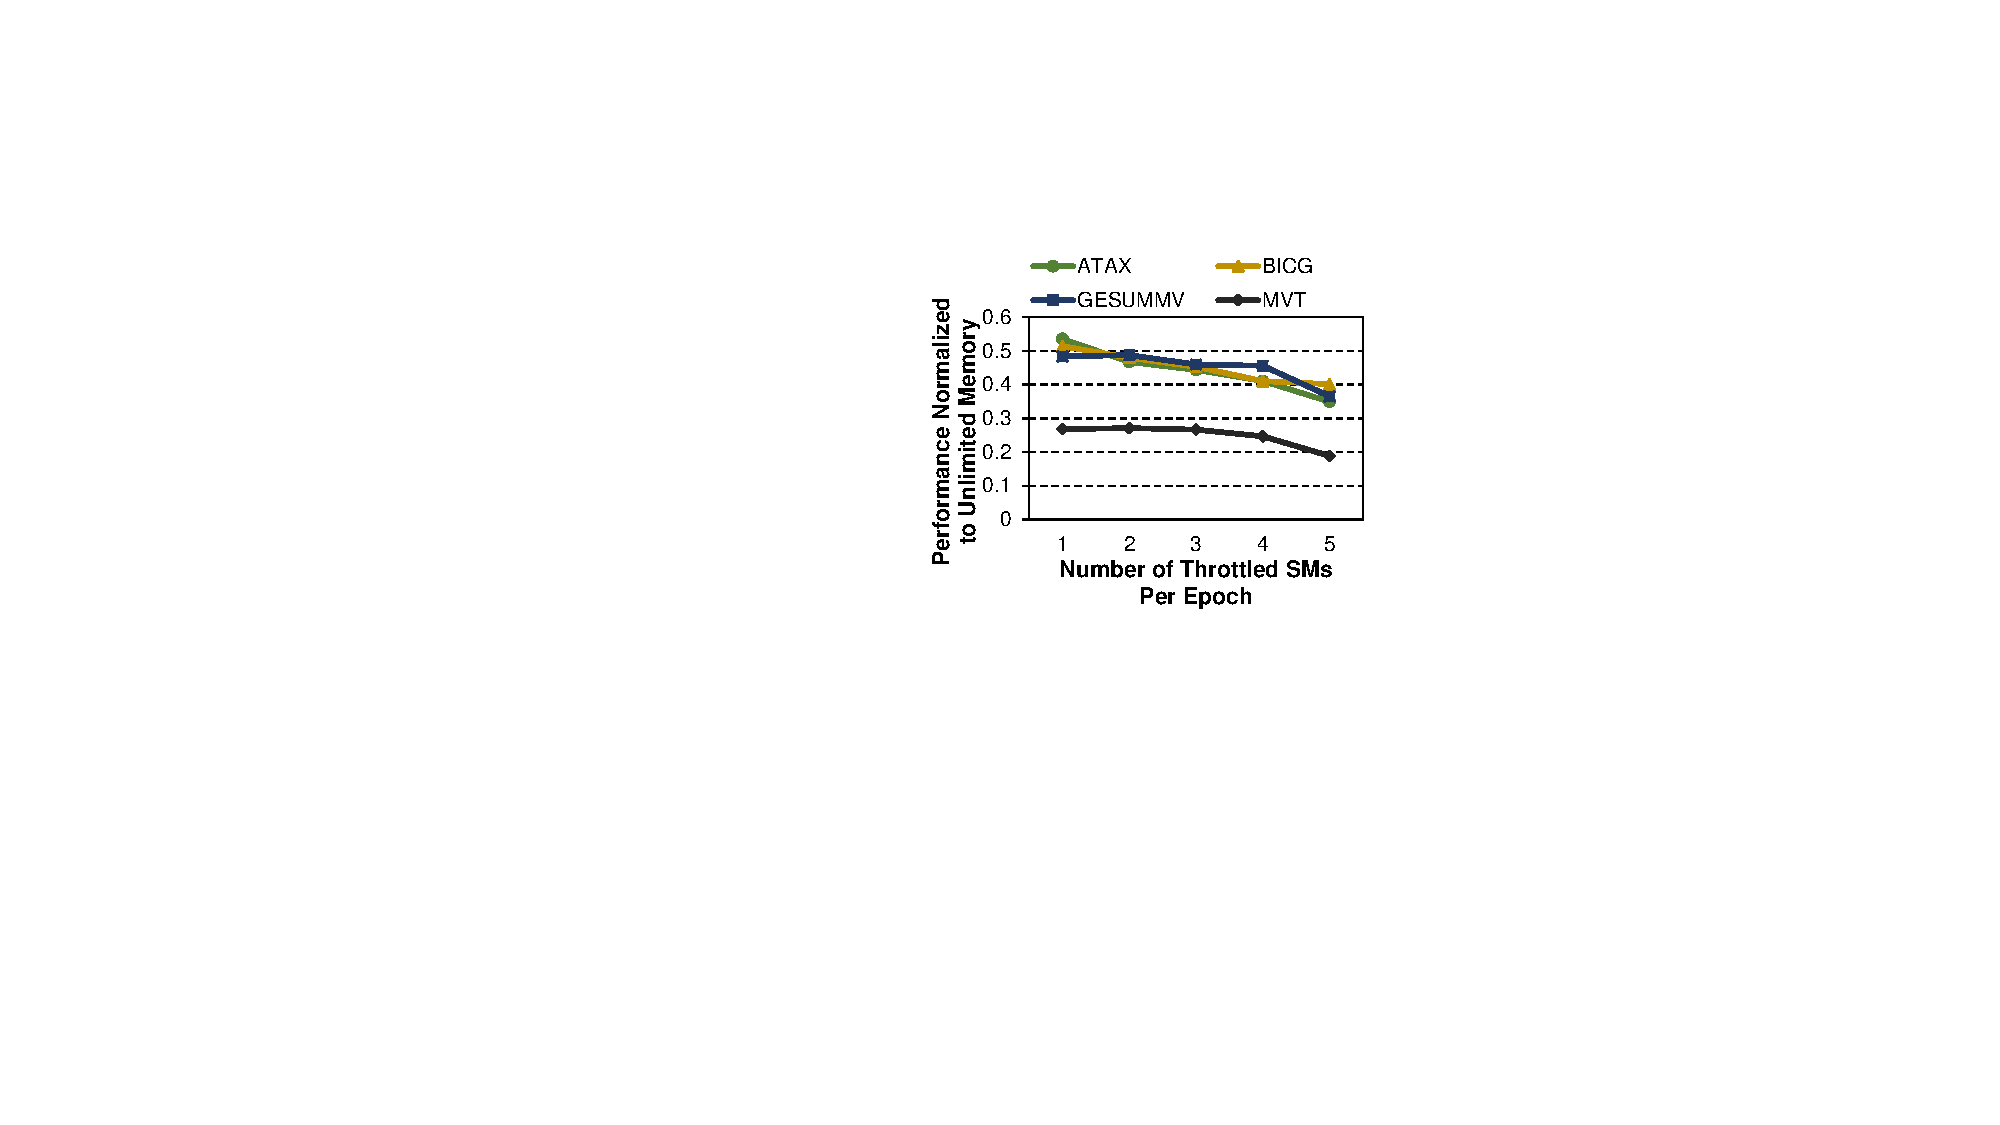
\includegraphics[width=.5\textwidth]{/Figs_ETC/data_throttle_SMs_sensitive}
  \caption{ETC的性能与减少GPU核心数量的关系}
  \label{fig:data_throttle_SMs_sensitive}
\end{figure}

\begin{figure}[htbp] % use float package if you want it here
  \centering
  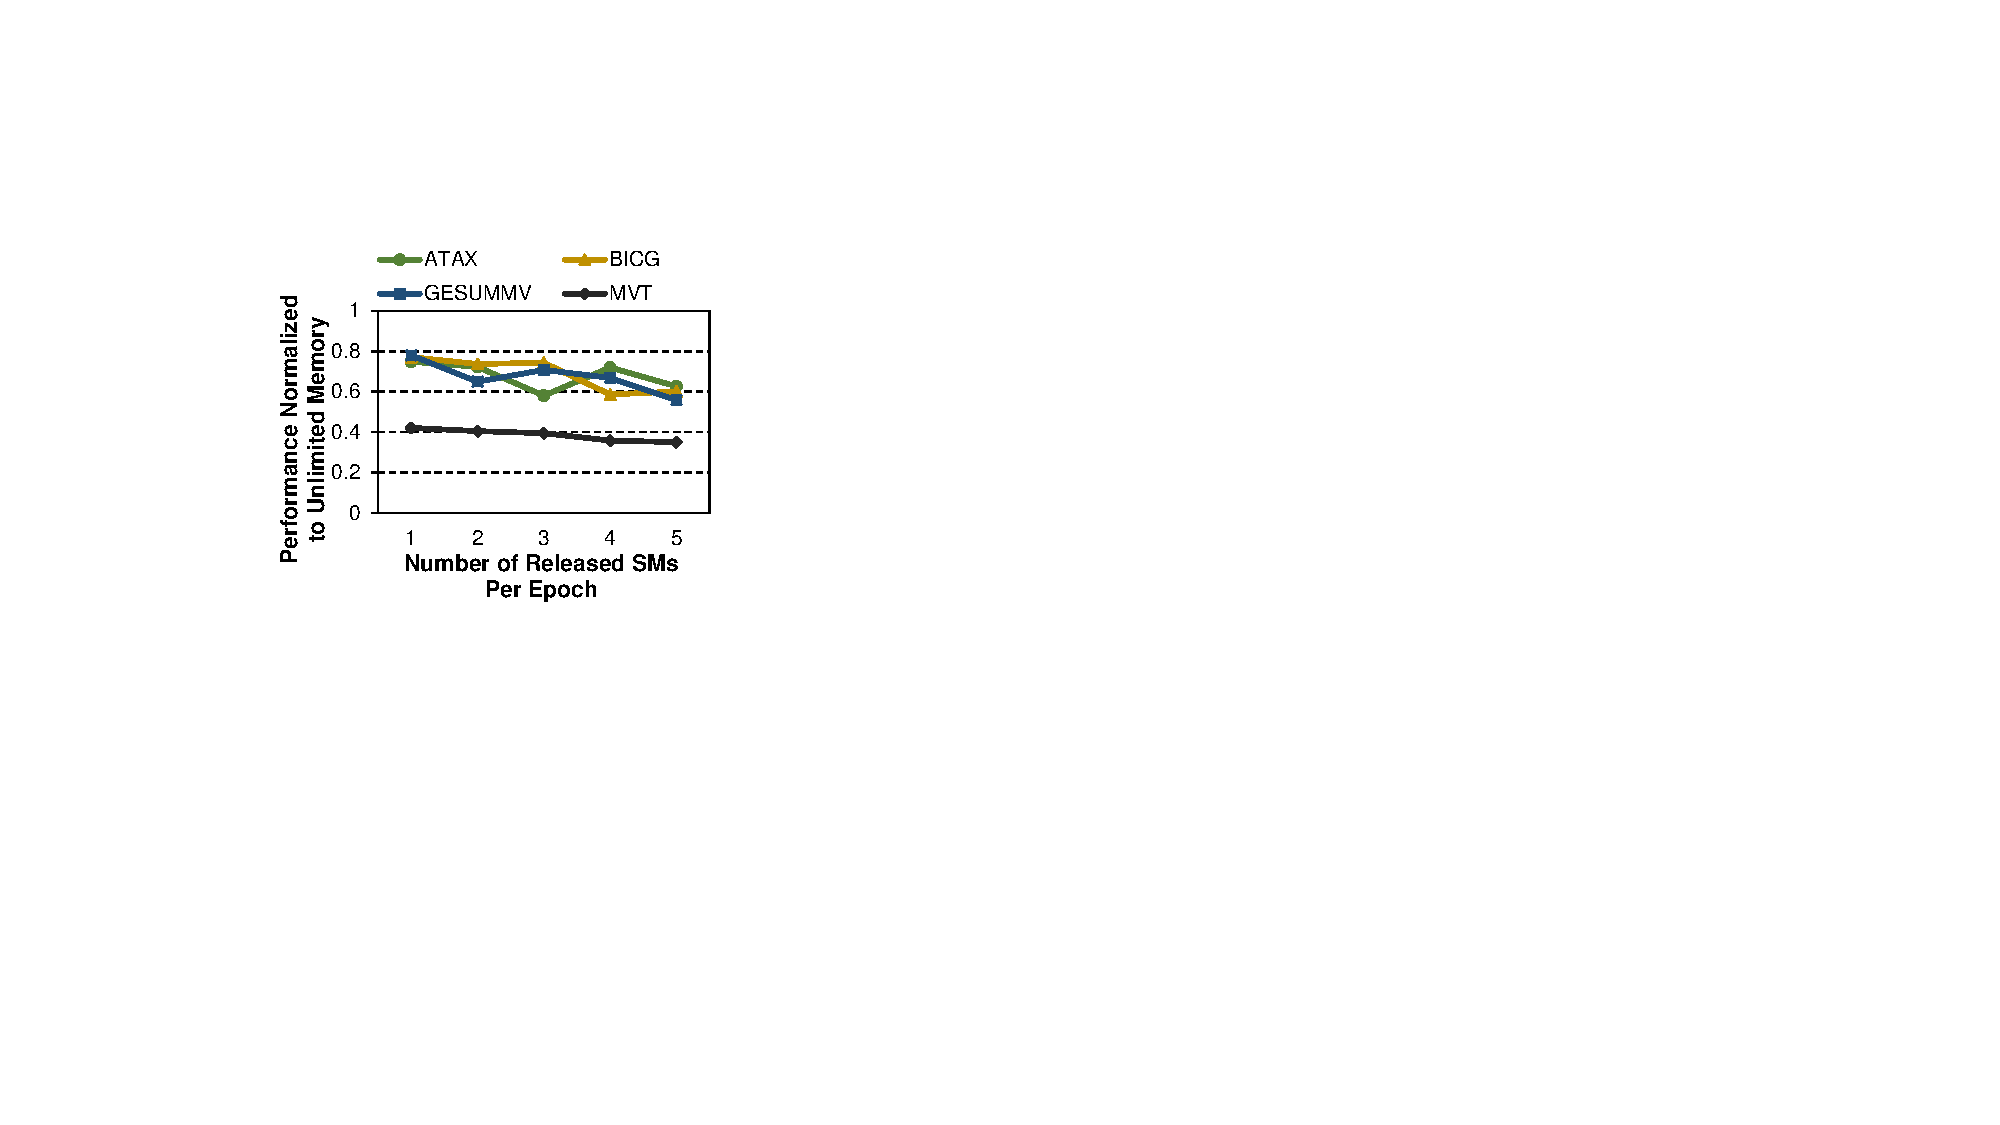
\includegraphics[width=.5\textwidth]{/Figs_ETC/data_release_SMs_sensitive}
  \caption{ETC的性能与增加GPU核心数量的关系}
  \label{fig:data_release_SMs_sensitive}
\end{figure}

\textbf{缺页中断延迟}。
图~\ref{fig:fault_latency}显示了GPGPU的应用程序在不同的缺页中断处理延迟下的性能。
实验设置缺页中断延迟从20$\mu$s到50$\mu$s不等。
实验结果显示的是相对于缺页中断延迟为20$\mu$s的性能。
我们观察到当缺页中断延迟从20$\mu$s提高到50$\mu$s,平均性能下降了31.2\%。
这些数据说明隐藏页逐出开销对于恢复内存超额配置下的性能非常重要,因为缺页中断延迟是主要的性能瓶颈。

\begin{figure}[htbp] % use float package if you want it here
  \centering
  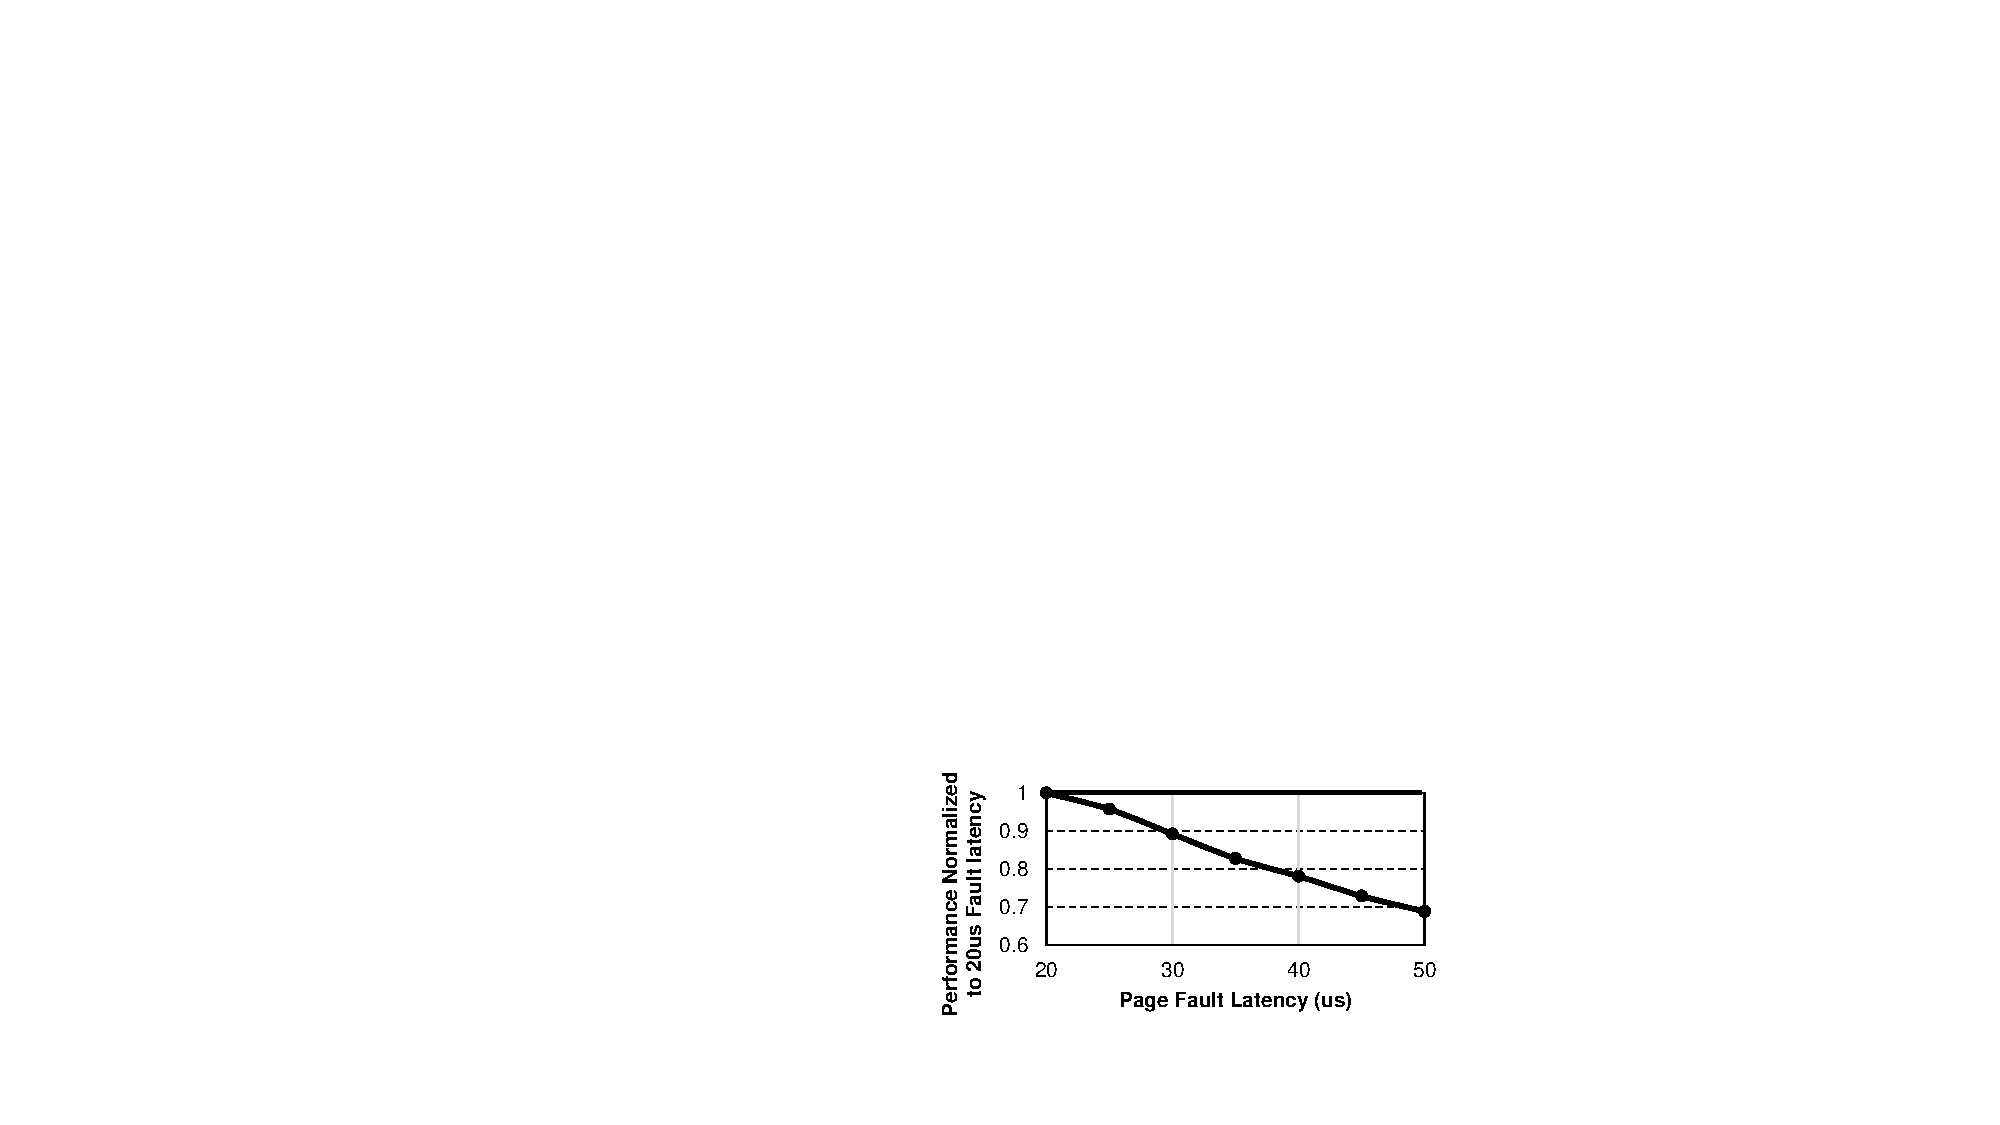
\includegraphics[width=.5\textwidth]{/Figs_ETC/fault_latency}
  \caption{ETC的性能与缺页中断延迟的关系}
  \label{fig:fault_latency}
\end{figure}

\textbf{压缩率}。
主存容量压缩技术影响到GPU主存能够容纳的数据页的数目。
图~\ref{fig:data_compression_ratio_sensitive}显示了所有应用程序采用不同的合成压缩率下的性能,相对于该应用在没有采用压缩技术的性能。
该实验在物理内存仅能容纳下50\%的内存占用的内存超额配置下进行。
实验结果显示GPU性能随着内存压缩率的增加而线性提高。
当所有的内存占用能够被GPU内存容纳时,性能有大幅度提升(压缩率为2)。

\begin{figure}[htbp] % use float package if you want it here
  \centering
  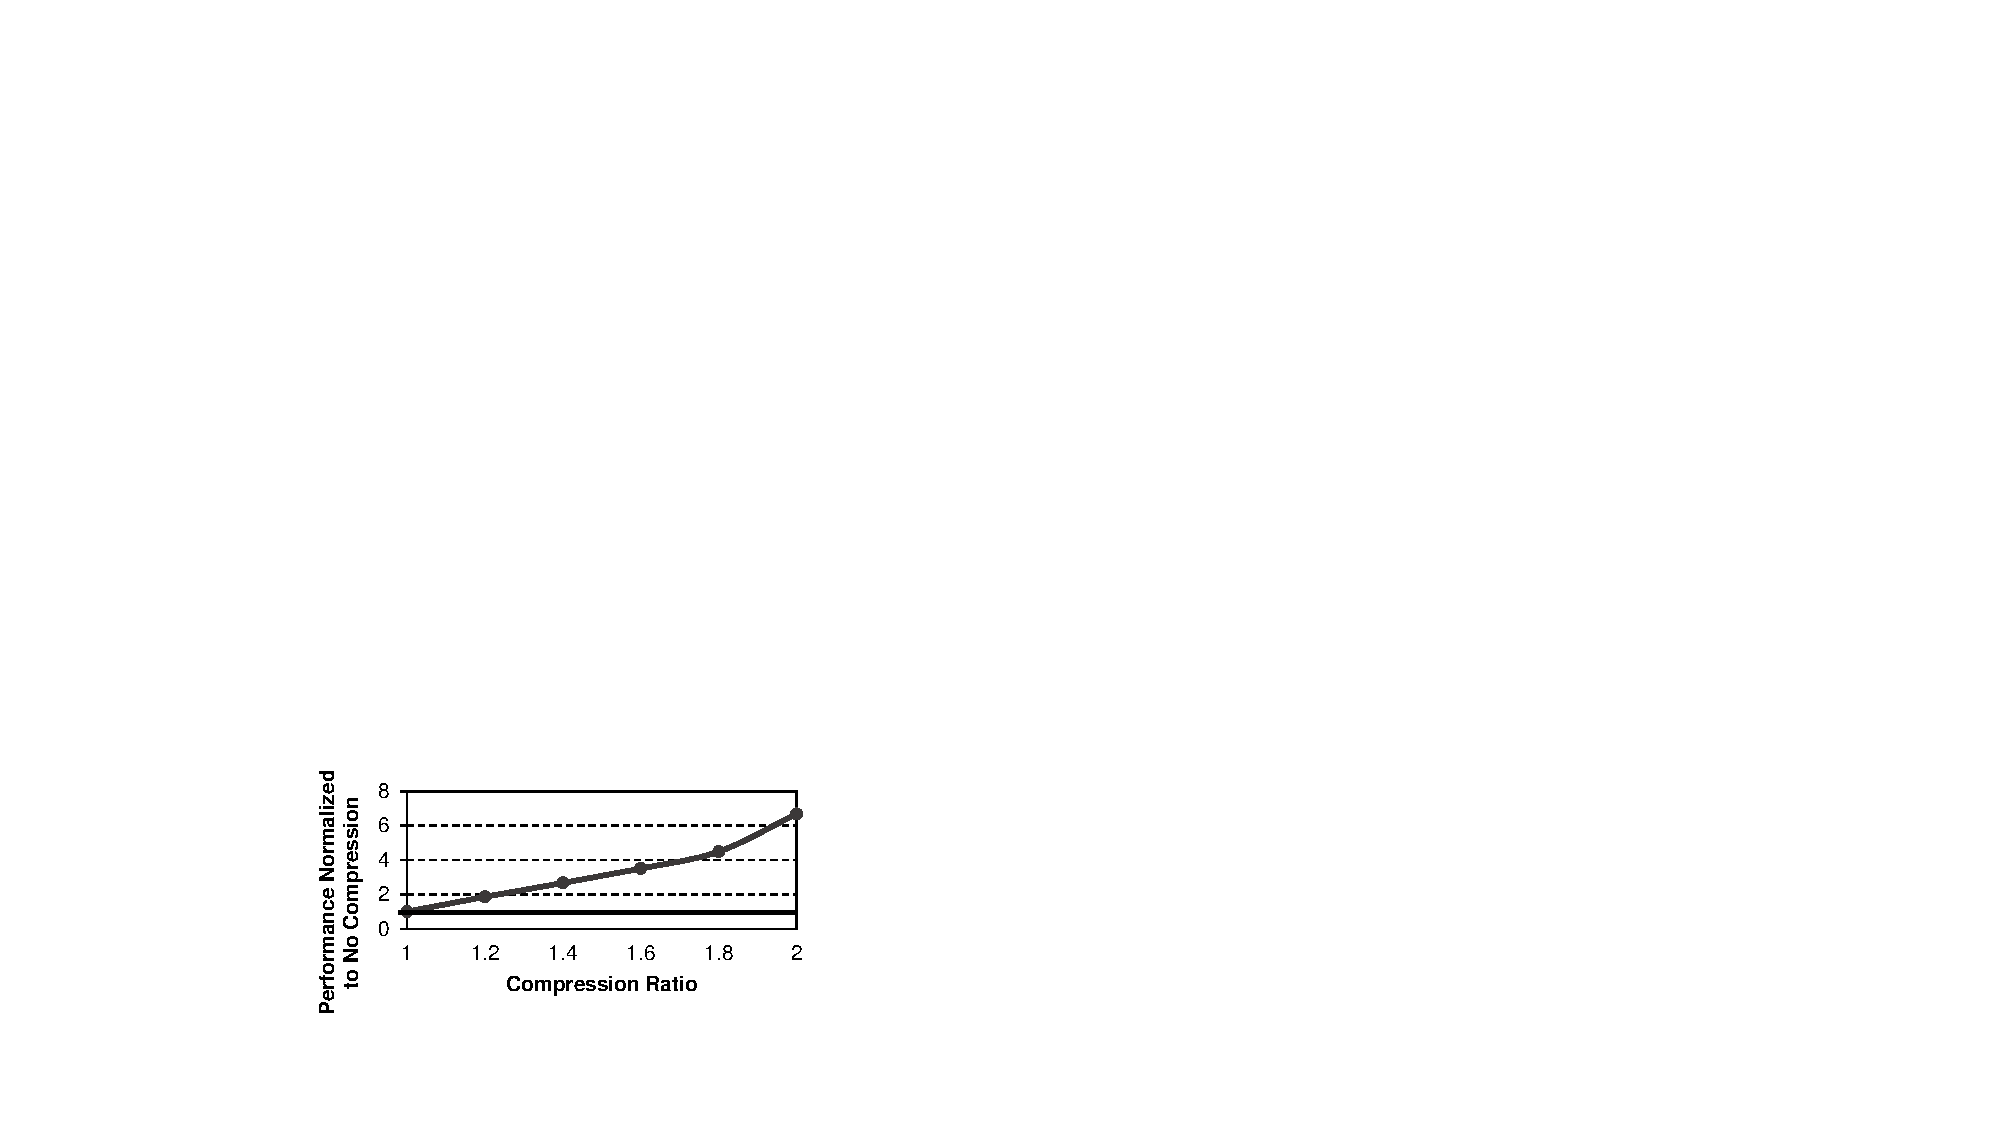
\includegraphics[width=.5\textwidth]{/Figs_ETC/data_compression_ratio_sensitive}
  \caption{ETC的性能与内存容量压缩率的关系}
  \label{fig:data_compression_ratio_sensitive}
\end{figure}

\subsection{硬件开销}
本章分析ETC框架的每个部分所耗费的硬件开销。
主动数据页逐出技术不需要任何硬件开销,可以直接在GPU驱动中实现。
我们修改了驱动来检测可用的内存大小以触发主动数据页逐出技术。
为实现内存感知的并行度控制技术,内存管理单元必须扩展以支持ETC设计。
增加两个32位的计数器来统计每个阶段的时钟周期。
暂停每个GPU核心的取指功能需要增加控制逻辑。
为实现容量压缩技术,本章增加的硬件开销和为CPU设计的LCP框类似,主要包括一个有512个条目的压缩元数据缓存。
内存压缩技术不需要额外的硬件开销,因为当前GPU已经具备了内存压缩和解压缩功能。
压缩与解压缩单元已经存在于存储控制器中~\upcite{rhu2018compressing,caba,kim2016bit}。
我们扩展页表项,每个页表项增加9位来包含压缩相关信息。
最后,应用程序划分单元需要:
(1)每个存取单元增加一个32位的访存合并计数器;
(2)连接取指单元,压缩单元以及内存管理控制器的信号控制线。
总的来说,我们的设计增加的硬件开销是有限的。
除了逻辑开销外,32KB的元数据缓存和482个32位计数器(30个GPU核心中每个GPU核心包含16个计数器,内存管理控制器有两个计数器),总存储开销小于2KB。

\section{本章小结}
\label{sec:etcconclusion}
本章介绍了ETC,一种在GPU中能够有效减少内存超额配置下的开销的内存管理框架。
该框架是对应用程序透明的,当内存超额配置情况下,规则应用程序和非规则应用程序呈现出不同的应用特性。
规则应用程序的性能受到数据页逐出延迟的影响非常大,而非规则应用程序的性能主要受到内存抖动的影响。
ETC划分应用程序为规则和非规则的类型,采用(1)主动数据页逐出技术来掩藏等待数据页逐出的延迟;
(2)内存感知的并行度控制技术来缓解内存抖动现象;
(3)内存容量压缩技术增加了有效内存容量。
对于无内存共享的规则应用程序,ETC消除了内存超额配置带来的性能损失,性能与无内存超额配置下类似。
对于数据共享的规则应用程序和非规则应用程序,ETC相比于当前技术,性能分别提升了60.4\%和270\%。
本章得出结论,ETC是一种高效低开销的框架,对于GPU内存超额配置开销最小化具有重要作用。

